% Options for packages loaded elsewhere
\PassOptionsToPackage{unicode}{hyperref}
\PassOptionsToPackage{hyphens}{url}
\PassOptionsToPackage{dvipsnames,svgnames,x11names}{xcolor}
\documentclass[
  11pt,
]{article}
\usepackage{xcolor}
\usepackage{amsmath,amssymb}
\setcounter{secnumdepth}{-\maxdimen} % remove section numbering
\usepackage{iftex}
\ifPDFTeX
  \usepackage[T1]{fontenc}
  \usepackage[utf8]{inputenc}
  \usepackage{textcomp} % provide euro and other symbols
\else % if luatex or xetex
  \usepackage{unicode-math} % this also loads fontspec
  \defaultfontfeatures{Scale=MatchLowercase}
  \defaultfontfeatures[\rmfamily]{Ligatures=TeX,Scale=1}
\fi
\usepackage{lmodern}
\ifPDFTeX\else
  % xetex/luatex font selection
\fi
% Use upquote if available, for straight quotes in verbatim environments
\IfFileExists{upquote.sty}{\usepackage{upquote}}{}
\IfFileExists{microtype.sty}{% use microtype if available
  \usepackage[]{microtype}
  \UseMicrotypeSet[protrusion]{basicmath} % disable protrusion for tt fonts
}{}
\makeatletter
\@ifundefined{KOMAClassName}{% if non-KOMA class
  \IfFileExists{parskip.sty}{%
    \usepackage{parskip}
  }{% else
    \setlength{\parindent}{0pt}
    \setlength{\parskip}{6pt plus 2pt minus 1pt}}
}{% if KOMA class
  \KOMAoptions{parskip=half}}
\makeatother
\usepackage{color}
\usepackage{fancyvrb}
\newcommand{\VerbBar}{|}
\newcommand{\VERB}{\Verb[commandchars=\\\{\}]}
\DefineVerbatimEnvironment{Highlighting}{Verbatim}{commandchars=\\\{\}}
% Add ',fontsize=\small' for more characters per line
\newenvironment{Shaded}{}{}
\newcommand{\AlertTok}[1]{\textcolor[rgb]{1.00,0.00,0.00}{\textbf{#1}}}
\newcommand{\AnnotationTok}[1]{\textcolor[rgb]{0.38,0.63,0.69}{\textbf{\textit{#1}}}}
\newcommand{\AttributeTok}[1]{\textcolor[rgb]{0.49,0.56,0.16}{#1}}
\newcommand{\BaseNTok}[1]{\textcolor[rgb]{0.25,0.63,0.44}{#1}}
\newcommand{\BuiltInTok}[1]{\textcolor[rgb]{0.00,0.50,0.00}{#1}}
\newcommand{\CharTok}[1]{\textcolor[rgb]{0.25,0.44,0.63}{#1}}
\newcommand{\CommentTok}[1]{\textcolor[rgb]{0.38,0.63,0.69}{\textit{#1}}}
\newcommand{\CommentVarTok}[1]{\textcolor[rgb]{0.38,0.63,0.69}{\textbf{\textit{#1}}}}
\newcommand{\ConstantTok}[1]{\textcolor[rgb]{0.53,0.00,0.00}{#1}}
\newcommand{\ControlFlowTok}[1]{\textcolor[rgb]{0.00,0.44,0.13}{\textbf{#1}}}
\newcommand{\DataTypeTok}[1]{\textcolor[rgb]{0.56,0.13,0.00}{#1}}
\newcommand{\DecValTok}[1]{\textcolor[rgb]{0.25,0.63,0.44}{#1}}
\newcommand{\DocumentationTok}[1]{\textcolor[rgb]{0.73,0.13,0.13}{\textit{#1}}}
\newcommand{\ErrorTok}[1]{\textcolor[rgb]{1.00,0.00,0.00}{\textbf{#1}}}
\newcommand{\ExtensionTok}[1]{#1}
\newcommand{\FloatTok}[1]{\textcolor[rgb]{0.25,0.63,0.44}{#1}}
\newcommand{\FunctionTok}[1]{\textcolor[rgb]{0.02,0.16,0.49}{#1}}
\newcommand{\ImportTok}[1]{\textcolor[rgb]{0.00,0.50,0.00}{\textbf{#1}}}
\newcommand{\InformationTok}[1]{\textcolor[rgb]{0.38,0.63,0.69}{\textbf{\textit{#1}}}}
\newcommand{\KeywordTok}[1]{\textcolor[rgb]{0.00,0.44,0.13}{\textbf{#1}}}
\newcommand{\NormalTok}[1]{#1}
\newcommand{\OperatorTok}[1]{\textcolor[rgb]{0.40,0.40,0.40}{#1}}
\newcommand{\OtherTok}[1]{\textcolor[rgb]{0.00,0.44,0.13}{#1}}
\newcommand{\PreprocessorTok}[1]{\textcolor[rgb]{0.74,0.48,0.00}{#1}}
\newcommand{\RegionMarkerTok}[1]{#1}
\newcommand{\SpecialCharTok}[1]{\textcolor[rgb]{0.25,0.44,0.63}{#1}}
\newcommand{\SpecialStringTok}[1]{\textcolor[rgb]{0.73,0.40,0.53}{#1}}
\newcommand{\StringTok}[1]{\textcolor[rgb]{0.25,0.44,0.63}{#1}}
\newcommand{\VariableTok}[1]{\textcolor[rgb]{0.10,0.09,0.49}{#1}}
\newcommand{\VerbatimStringTok}[1]{\textcolor[rgb]{0.25,0.44,0.63}{#1}}
\newcommand{\WarningTok}[1]{\textcolor[rgb]{0.38,0.63,0.69}{\textbf{\textit{#1}}}}
\usepackage{longtable,booktabs,array}
\newcounter{none} % for unnumbered tables
\usepackage{calc} % for calculating minipage widths
% Correct order of tables after \paragraph or \subparagraph
\usepackage{etoolbox}
\makeatletter
\patchcmd\longtable{\par}{\if@noskipsec\mbox{}\fi\par}{}{}
\makeatother
% Allow footnotes in longtable head/foot
\IfFileExists{footnotehyper.sty}{\usepackage{footnotehyper}}{\usepackage{footnote}}
\makesavenoteenv{longtable}
% definitions for citeproc citations
\NewDocumentCommand\citeproctext{}{}
\NewDocumentCommand\citeproc{mm}{%
  \begingroup\def\citeproctext{#2}\cite{#1}\endgroup}
\makeatletter
 % allow citations to break across lines
 \let\@cite@ofmt\@firstofone
 % avoid brackets around text for \cite:
 \def\@biblabel#1{}
 \def\@cite#1#2{{#1\if@tempswa , #2\fi}}
\makeatother
\newlength{\cslhangindent}
\setlength{\cslhangindent}{1.5em}
\newlength{\csllabelwidth}
\setlength{\csllabelwidth}{3em}
\newenvironment{CSLReferences}[2] % #1 hanging-indent, #2 entry-spacing
 {\begin{list}{}{%
  \setlength{\itemindent}{0pt}
  \setlength{\leftmargin}{0pt}
  \setlength{\parsep}{0pt}
  % turn on hanging indent if param 1 is 1
  \ifodd #1
   \setlength{\leftmargin}{\cslhangindent}
   \setlength{\itemindent}{-1\cslhangindent}
  \fi
  % set entry spacing
  \setlength{\itemsep}{#2\baselineskip}}}
 {\end{list}}
\usepackage{calc}
\newcommand{\CSLBlock}[1]{\hfill\break\parbox[t]{\linewidth}{\strut\ignorespaces#1\strut}}
\newcommand{\CSLLeftMargin}[1]{\parbox[t]{\csllabelwidth}{\strut#1\strut}}
\newcommand{\CSLRightInline}[1]{\parbox[t]{\linewidth - \csllabelwidth}{\strut#1\strut}}
\newcommand{\CSLIndent}[1]{\hspace{\cslhangindent}#1}
\setlength{\emergencystretch}{3em} % prevent overfull lines
\providecommand{\tightlist}{%
  \setlength{\itemsep}{0pt}\setlength{\parskip}{0pt}}
% Extra preamble: Unicode characters used in the report body that plain
% pdflatex + inputenc(utf8)/fontenc(T1) do not already cover.
\DeclareUnicodeCharacter{0394}{\ensuremath{\Delta}}     % Δ
\DeclareUnicodeCharacter{03C0}{\ensuremath{\pi}}        % π
\DeclareUnicodeCharacter{03C1}{\ensuremath{\rho}}       % ρ
\DeclareUnicodeCharacter{03C9}{\ensuremath{\omega}}     % ω
\DeclareUnicodeCharacter{2191}{\ensuremath{\uparrow}}   % ↑
\DeclareUnicodeCharacter{2192}{\ensuremath{\rightarrow}}% →
\DeclareUnicodeCharacter{2193}{\ensuremath{\downarrow}} % ↓
\DeclareUnicodeCharacter{2208}{\ensuremath{\in}}        % ∈
\DeclareUnicodeCharacter{2212}{\ensuremath{-}}          % − (minus sign)
\DeclareUnicodeCharacter{2213}{\ensuremath{\mp}}        % ∓
\DeclareUnicodeCharacter{2248}{\ensuremath{\approx}}    % ≈
\DeclareUnicodeCharacter{2264}{\ensuremath{\leq}}       % ≤
\DeclareUnicodeCharacter{2265}{\ensuremath{\geq}}       % ≥

% Tables in the report are wider than the 1in-margin textwidth in places;
% allow small tables to shrink to fit rather than overflow.
\usepackage{adjustbox}

% Long inline results/*.json paths in \texttt{} (Appendix C/D/E artifact
% lists) have no natural break point; allow breaking at underscores/hyphens
% so they wrap instead of overflowing the margin.
\usepackage[htt]{hyphenat}

% Long, evidence-heavy paragraphs run pages before the next figure; keep
% figures near their reference point without forcing a hard float barrier.
\usepackage{float}

% [H] forces a figure to its exact source position even when it doesn't fit
% on the current page, leaving a large blank gap instead of flowing text
% around it. placeins' \FloatBarrier lets a figure float naturally ([htbp])
% while still forbidding it from drifting past a given point (e.g. past its
% own section), avoiding both the drift and the forced-gap failure modes.
\usepackage{placeins}

% Appendix A's verbatim prompt text has long lines; pandoc's fenced-code
% Highlighting environment (fancyvrb Verbatim) doesn't wrap by default,
% which overflows the page margin. Wrap and shrink it slightly instead.
\usepackage{fvextra}
\DefineVerbatimEnvironment{Highlighting}{Verbatim}{commandchars=\\\{\},breaklines=true,breakanywhere=true,fontsize=\small}

% Bullets (e.g. the metric definitions in 3.4) often contain long inline
% `code` spans -- pandoc renders their internal spaces as fixed-width \
% control spaces, so the whole span is one unbreakable chunk near a full
% line's width. Under full justification, LaTeX compensates by stretching
% the few remaining breakable spaces on that line unevenly. Ragged-right
% itemize lets the leftover space fall to the margin instead.
\AtBeginEnvironment{itemize}{\raggedright}
% Loaded after preamble.tex (and after pandoc's font setup) so that
% arxiv.sty's Times/Helvetica font selection and its own \newgeometry
% (set in \AtBeginDocument) win over pandoc's defaults.
\usepackage{arxiv}

% arxiv.sty itself sets \flushbottom, which combined with the template's
% stretchy \parskip stretches interline space to fill short pages exactly,
% producing large visible gaps above/below figures on pages with few
% paragraphs (e.g. Figure 1 on a page ending right after a section break).
% Override back to \raggedbottom so pages end short instead.
\raggedbottom

% arxiv.sty's default \shorttitle is the full \@title, which collides with
% the right-aligned "A Preprint" running header for a title this long.
\renewcommand{\shorttitle}{Reasoning-to-Execution Gap in LLM Agents}

% body.md frequently nests a \subsection directly under a \section with no
% lead-in paragraph between them (each section is a container for its
% subsections). arxiv.sty's stock spacing (section after-skip 1.5ex,
% subsection before-skip -1.8ex) is tuned for headings separated by body
% text; back-to-back headings collapse into one visual blob under it. Widen
% both so a section-then-subsection pair reads as two distinct breaks,
% matching the whitespace in the upstream arxiv-style template.pdf.
% \@startsection/\z@/\@plus/\@minus below need catcode-11 "@", which .sty
% files get automatically but a plain --include-in-header snippet does not.
\makeatletter
\renewcommand{\section}{%
  \@startsection{section}{1}{\z@}%
                {-2.5ex \@plus -0.5ex \@minus -0.2ex}%
                { 2.3ex \@plus  0.3ex \@minus  0.2ex}%
                {\large\bf\raggedright}%
}
\renewcommand{\subsection}{%
  \@startsection{subsection}{2}{\z@}%
                {-3.0ex \@plus -0.5ex \@minus -0.2ex}%
                { 1.0ex \@plus  0.2ex}%
                {\normalsize\bf\raggedright}%
}
\makeatother
\usepackage{bookmark}
\IfFileExists{xurl.sty}{\usepackage{xurl}}{} % add URL line breaks if available
\urlstyle{same}
\hypersetup{
  pdftitle={Diagnosing and Reducing the Reasoning-to-Execution Gap in LLM Sequential Decision Agents},
  colorlinks=true,
  linkcolor={black},
  filecolor={Maroon},
  citecolor={black},
  urlcolor={black},
  pdfcreator={LaTeX via pandoc}}

\title{Diagnosing and Reducing the Reasoning-to-Execution Gap in LLM Sequential Decision Agents}
\author{Vincent Marciano Fan\\
HKUST\\
vmfan@connect.ust.hk}
\date{}

\begin{document}
\maketitle
\begin{abstract}
LLM agents in sequential decision settings often fail at \emph{doing}, not \emph{knowing}: they can state a correct belief and still take an action that belief does not justify. Existing harness-reliability metrics cannot see this: they check whether an action was correct, not whether it was consistent with the agent's own stated reasoning, because realistic settings have no ground-truth optimal action to check against. We build a minimal repeated-pricing game small enough to admit an \emph{exact} EV oracle, paired with same-pass belief elicitation, giving a two-oracle decomposition of failure into \textbf{estimation error} (Oracle B: is the stated belief close to the correct posterior?) and \textbf{execution error} (Oracle A: does the chosen action follow from the agent's own stated belief?). On a weak model (Llama 3.3 70B) both channels are severely broken (directional agreement 0.524, barely above chance; mean EV-realization ratio −0.369, 61\% of decisions realize negative EV). Capability does not close the gap, but relocates it. The frontier model (GPT-5.5) has largely correct beliefs (TV distance 0.063, directional agreement 0.945) but still forfeits value on 66\% of decisions relative to its own stated belief (mean ratio 0.893). We then test a no-training scaffold, an externalized belief-state carry plus a mandated re-evaluation step, against a token-matched control that isolates structure from reasoning budget. The scaffold does not close the gap either: on the frontier it \emph{widens} the estimation-error axis, worst on the belief-carry component (TV 0.088 vs.~0.052 for the control), a mechanism we trace to double-counting of already-summarized evidence and confirm with a signed over-concentration fingerprint, replicated on an independent frontier model. A follow-up fix, replacing raw history with its lossless sufficient statistic, repairs the belief axis (lowest estimation error of any arm, both models) at \emph{negative} token cost. But a composite true-model decision-quality metric shows this belief win is largely cosmetic on the frontier (all arms ≈0.93) and dissociates from decision quality on the weak model, where a different, cheap intervention (de-duplicated belief-carry) delivers the largest gain in the study (+0.224, 1.14 quality-points per 1K extra tokens) despite worse beliefs than the sufficient-statistic arm. The takeaway is that a validated instrument separating estimation from execution error is necessary to see that a plausible, cheap scaffold can degrade the axis it targets while leaving decisions unchanged, and that ``better beliefs'' and ``better decisions'' are not the same intervention.
\end{abstract}

\section{1\quad Introduction}\label{introduction}

Autonomous LLM agents are increasingly evaluated on a semantic gap between what they \emph{intend} and what they \emph{do}: whether a plan, a stated constraint, or a declared belief is actually reflected in the action the agent takes next. This gap has been documented as a reliability problem in tool-use and embodied harnesses (ActPlane {[}28{]}, detailed in §2.1): agents that reason correctly in one turn can still emit an action in the next that violates their own stated reasoning.

This project studies that failure class directly, in a setting deliberately built to make it exact rather than anecdotal. LLM agents in sequential decision settings fail at \emph{doing}, not \emph{knowing}: an agent can state the correct belief about its environment and still choose an action that belief does not justify. In our setting, a repeated market-making game, this shows up as concrete, nameable failure signatures: unjustified conservatism (quoting wider or smaller than the agent's own stated belief implies), belief staleness after a fill (failing to update the next quote on new evidence the agent has already observed), and optimistic counterparty modeling (treating flow as uninformed when the agent's own stated belief says otherwise).

Existing harness-reliability metrics are structurally blind to this failure class. Work in this space measures whether an agent's action was \emph{correct}, for example a Decision Compliance Rate that flags whether a violation occurred, but in realistic tool-use or embodied settings there is no ground-truth optimal action to check the agent's choice against. That makes it impossible to distinguish ``the agent could not have complied'' (a capability limit) from ``the agent could have complied but did not'' (an execution failure): precisely the distinction that matters for deciding whether a fix belongs in the model, the prompt, or the scaffold.

This project's move is to trade a realistic environment for one small enough to admit an \emph{exact} optimal-action oracle, and to elicit the agent's belief in the same pass as its action. That combination decomposes failure into two orthogonal, independently measurable quantities: estimation error (is the agent's stated belief close to the environment's true posterior?) and execution error (does the agent's chosen action follow from \emph{its own} stated belief, regardless of whether that belief is correct?). Because both oracles are exact and both scores are computed against the same elicited object, this measures whether an agent acts consistently with its own stated reasoning, not merely whether it acts correctly.

We use this instrument to test a no-training scaffold designed to fix execution error: an externalized belief-state carry (the agent's posterior from the previous round is re-injected verbatim) plus a mandated re-evaluation step before each action. Because chain-of-thought alone is known to change outcomes independent of any structural change, we measure the scaffold's effect against a token-matched control that reproduces its reasoning budget without its structure, so a positive or null result cannot collapse into ``more tokens helps'' or ``CoT helps.'' The scaffold is evaluated \emph{through} the validated two-oracle instrument, not against a proxy metric, so its effect can be attributed to the specific axis (belief formation vs.~belief-to-action follow-through) it changes.

This paper makes three contributions:

\begin{itemize}
\tightlist
\item
  \textbf{C-a.} A validated, frozen diagnostic instrument, a two-oracle decomposition (exact EV oracle + exact posterior oracle) plus same-pass belief elicitation, that separates estimation error from execution error with closed-form ground truth (§3).
\item
  \textbf{C-b.} A quantified reasoning-to-execution gap on both a weak model (Llama 3.3 70B) and a frontier model (GPT-5.5), showing the gap persists at the frontier but relocates from estimation to execution as capability increases (§5, RQ1--RQ2).
\item
  \textbf{C-c.} A component-attributed scaffold effect against a token-matched control, reported jointly with token, latency, and dollar cost, showing the scaffold degrades the axis it targets rather than fixing it, diagnosing the mechanism, and testing a follow-up fix (§5, RQ3--RQ4).
\end{itemize}

\section{2\quad Motivation}\label{motivation}

\subsection{2.1\quad Knowing--doing failures in agent harnesses}\label{knowingdoing-failures-in-agent-harnesses}

This project's failure class is a documented reliability problem that has not yet been measured directly. Motivated by evidence that agents comply with instructions only \emph{probabilistically}, ActPlane {[}28{]} targets exactly this operational hazard: a correctly-stated constraint is violated on a nontrivial fraction of turns even when nothing about the environment prevents compliance, but its Decision Compliance Rate reports whether a violation occurred, not how far the chosen action was from the best one, because no ground-truth optimum is available in its task suite. ActPlane treats the gap as an operational hazard to be contained, but does not decompose it into ``the agent believed the wrong thing'' versus ``the agent believed the right thing and acted on something else.''

That two-layer decomposition (state-tracking failure vs.~execution failure) is the axis this project measures directly, and the severity is not subtle once an exact oracle makes it visible. An unscaffolded pilot run (§3.5) found both the frontier model (GPT-5.5) and the weak model (Llama 3.3 70B) leaving value on the table against their own stated beliefs, the EV-realization ratio defined formally in §3.4. The weak model's policy realized \emph{negative} expected value on average, worse than not trading at all, judged purely by whether it followed its own stated reasoning. This is a severe result by any standard: a model can state a belief and then act against it so consistently that its policy has negative expected value under its own accounting. §5 shows this severity holds up at N=145 evidence-bearing decisions (not just the N=8 pilot) and further decomposes it into estimation error and execution error.

\subsection{2.2\quad Why measurement requires a minimal game}\label{why-measurement-requires-a-minimal-game}

A natural objection: why not measure this reasoning-to-execution gap on a realistic agent benchmark (OS-level tasks, coding harnesses, tool-use pipelines) rather than a market-making toy?

The answer follows directly from what execution error requires to be well-defined. Execution error is the gap between an agent's chosen action and the EV-optimal action \emph{under that agent's own stated belief}. Computing that gap requires an oracle that returns the exact optimal action for any belief: not an approximation, not an LLM judge, not a Monte Carlo estimate, because approximation error in the oracle would be indistinguishable from execution error in the agent, and the entire measurement would collapse. No such oracle exists for OS-level or coding tasks: this is precisely why harness-reliability work in this space, for example ActPlane's Decision Compliance Rate, scores whether a violation occurred (a pass/fail compliance check) rather than whether the chosen action was optimal. That is not a limitation of prior work, but the reason the reasoning-to-execution gap has gone unmeasured. A harness rich enough to be realistic is a harness too rich for an exact oracle.

So the environment here is sized backward from the oracle, not forward from realism: the repeated-pricing game is the smallest environment that still contains all three structural features the gap requires, information that keeps arriving after an action is taken (so belief staleness is even definable), an action space with a magnitude dimension (so conservatism is measurable, not just a binary choice), and a counterparty type inferable from observed flow (so there is an adverse-selection cost to being naive about). Remove any one of the three and the corresponding failure mode becomes structurally unmeasurable, no matter how the LLM behaves.

Two further design consequences follow from taking the oracle-exactness constraint seriously, not incidentally. First, rounds may be coupled through what the agent should believe, never through what is mechanically optimal to do (banning hard inventory limits and any information-value-of-trading effect), because any such control coupling would make the true optimal action depend on future rounds or past actions, breaking the myopic one-round oracle that keeps the computation exact and cheap. Second, the resulting state space, a ternary hidden value, two counterparty types, a six-round horizon, is small enough that both oracles' optimal actions can be hand-computed and independently verified (Appendix B), which is what makes the instrument's validity checkable rather than merely asserted.

This has an empirical answer, not just an a priori one: is the resulting game actually solvable, or has minimality made it degenerate? A simple Bayesian heuristic agent (correct posterior update, EV-greedy action selection, no learning, no scaffold) reaches the EV-realization ceiling (ratio 1.0) on all 48 of 48 decisions at the frozen horizon, using the same sanity-baseline control described in §3.5. The task is mechanically solvable by a policy with no more sophistication than exact Bayesian updating plus greedy EV maximization. Any gap measured in an LLM agent against this same ceiling is therefore a real finding about the agent, not an artifact of an impossibly hard or degenerate task.

The game, in short, is the price paid for measurement precision, not the object of study: a diagnostic instrument for a specific internal mechanism (does an agent act on its own stated beliefs), not a trading system and not a general-purpose benchmark.

\section{3\quad The Instrument}\label{the-instrument}

\subsection{3.1\quad Environment: a minimal repeated-pricing game}\label{environment-a-minimal-repeated-pricing-game}

Each episode has one hidden asset value \texttt{V}, drawn uniformly at the start of the episode from \texttt{\{10,\ 15,\ 20\}} and fixed for the whole episode; \texttt{V} is revealed only once the episode ends. Over a fixed horizon of \texttt{H\ =\ 6} rounds, one counterparty arrives per round to trade against the agent's quotes. Each counterparty is one of two types, never revealed to the agent: \emph{informed} counterparties know \texttt{V} and trade in its direction (buy if \texttt{V=20}, sell if \texttt{V=10}, 50/50 if \texttt{V=15}); \emph{uninformed} counterparties trade 50/50 regardless of \texttt{V}. Types are drawn independently per arrival at a fixed, undisclosed rate.

Each round, in a single forward pass (§3.3), the agent states a posterior over \texttt{V} and over the informed-arrival share, then chooses an action: a spread (tight/medium/wide, half-width 1/2/3 around the midpoint implied by its own stated belief) and a size (1, 2, or 3 units). A trade completes probabilistically, less often as spread widens and size grows, more steeply so for uninformed counterparties than informed ones, and settles at episode end against the true \texttt{V}.

The horizon (\texttt{H=6}) sits within the pre-registered two-way-door range, chosen because a shorter horizon leaves too little headroom: at \texttt{H=4}, both models tested were EV-optimal on every round-1 and round-2 decision, leaving only \textasciitilde7\% of headroom on the frontier arm for rounds 3--4 to carry the entire measurable gap. Rounds ≥3 are exactly where a stated posterior has accumulated enough evidence to go stale, the phenomenon the intervention targets, so a longer horizon buys diagnostic signal where the gap actually lives, rather than changing anything about what is being measured.

Two kinds of cross-round dependence are possible in this design, and only one is permitted. Inference coupling, where earlier fills and observed flow change what the agent \emph{should believe} later, is required: without it, belief staleness has no meaning. Control coupling, where anything earlier changes what action is \emph{mechanically optimal} later independent of belief, such as a hard inventory limit or a value to trading purely for its informational effect, is banned. The reason is architectural: the action-EV oracle (§3.2) is myopic, computing the single best action for the round in front of it given the agent's stated belief, and myopic is what keeps the oracle exact and cheap to evaluate. It is only \emph{correct} as an oracle when the best action in any round is a function of current belief alone, so the only thing carried across rounds, by construction, is what the agent should believe, never what it is mechanically optimal to do.

\begin{figure}[H]
\centering
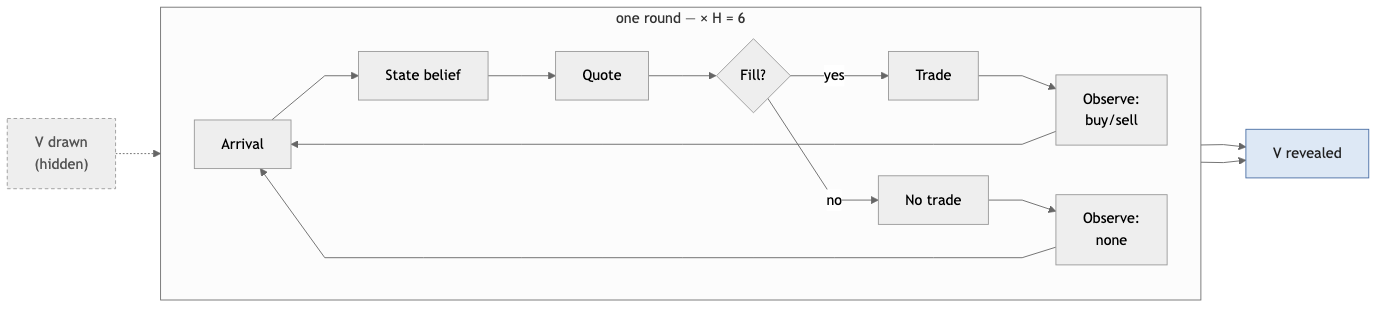
\includegraphics[width=0.85\textwidth]{results/fig_episode_timeline.png}
\caption{episode timeline. Arrival, quote, fill/no-fill, flow-direction observation, next round, looping \texttt{H=6} times before \texttt{V} is revealed.}
\label{fig:1}
\end{figure}

\subsection{3.2\quad The two-oracle decomposition}\label{the-two-oracle-decomposition}

The reasoning-to-execution decomposition rests on two oracles that answer two different questions about the same decision.

\textbf{Oracle A: action-EV given the agent's own stated belief.} For any candidate action, Oracle A computes its expected one-round PnL in closed form, conditioned on the agent's \emph{full} elicited belief state: its stated posterior over \texttt{V} and its stated informed-arrival share \texttt{ω} (\texttt{belief\_informed\_share}). Every quantity the agent actually states is substituted into the calculation, while only environment mechanics the agent was never asked to state (the fill-probability table, the type-conditional buy/sell rule) remain at their true values, since those are not beliefs the metric can hold the agent accountable for. The EV-optimal action under this belief, \texttt{a*\ =\ argmax\_a\ EV(a\ \textbar{}\ stated\ belief,\ ω)}, defines \textbf{execution error}: whether the agent took the action its own stated beliefs actually justify, independent of whether those beliefs were themselves correct.

\textbf{Oracle B: the true-model Bayes-optimal policy.} Oracle B solves the finite-horizon belief-state problem by exact backward induction under the \emph{true} prior and counterparty model, yielding both a PnL ceiling and the correct posterior trajectory. Comparing the agent's stated trajectory against this correct one defines \textbf{estimation error}: how far the agent's beliefs are from what a perfect Bayesian reasoner, seeing the same observations, would have concluded.

Oracle A asks ``did the agent act on its beliefs?''; Oracle B asks ``were those beliefs right?'' Neither question alone is answerable from harness-reliability metrics like Decision Compliance Rate, which score whether the action taken was permissible but have no ground-truth optimal action to compare against; the combination of both oracles against the same decision is exactly what such metrics cannot produce. Figure\textasciitilde{}\ref{fig:2} summarizes this decomposition: one stated belief feeding two oracles, producing two independent error channels.

\begin{figure}[H]
\centering
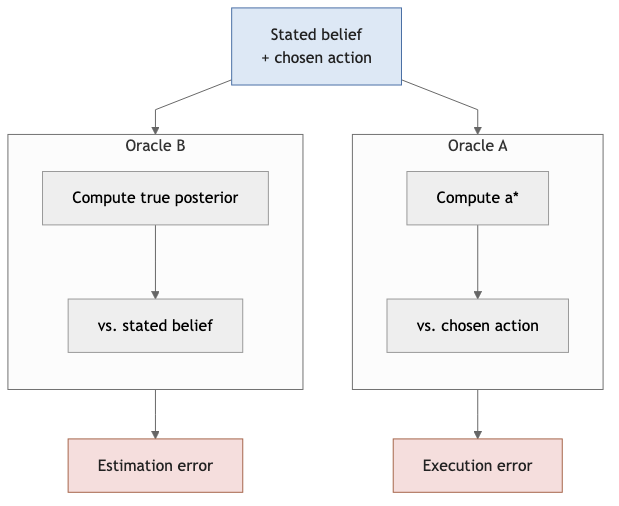
\includegraphics[width=0.5\textwidth]{results/fig_two_oracle.png}
\caption{belief, then two oracles, then two error channels: the report's central diagram.}
\label{fig:2}
\end{figure}

The EV-optimal action is belief-dependent rather than a fixed constant, because quoting wider earns more per completed trade but fills less often, while quoting tighter fills more often but at worse terms, exactly when an informed counterparty's information advantage is highest. This adverse-selection cost is captured by a haircut \texttt{c}, computed from the agent's own stated \texttt{V}-posterior, that is subtracted from the informed-counterparty term of the EV calculation. \texttt{c} is maximal when the agent's belief is diffuse and shrinks as the belief concentrates, since an agent that has inferred \texttt{V} is likely high or low has effectively caught up to the informed trader and can afford to tighten its quotes and size up. This is what makes the EV-optimal action move with belief: at a uniform prior (Node A) the optimum is a defensive \texttt{(wide,\ size\ 1)}; after evidence concentrates the posterior (Node B), it shifts to \texttt{(medium,\ size\ 2)}. Both oracles are held to exactness, closed-form for Oracle A, exact backward induction for Oracle B, rather than Monte Carlo approximation, and are verified against three hand-computed nodes and asserted as full 9-action EV vectors, not just argmax labels, in unit tests (Appendix B).

\subsection{3.3\quad Same-pass belief elicitation}\label{same-pass-belief-elicitation}

The EV-realization metric is only meaningful if the belief it conditions on is the belief the agent actually acted on. If belief and action were elicited in separate calls, nothing would guarantee the second call's action was conditioned on the first call's stated belief rather than some other internal state: the execution-error channel would be measuring the gap between two different beliefs, not between one belief and its own action. Belief and action are therefore elicited in a single forward pass: one structured JSON response per round, with the belief fields (\texttt{belief\_v}, \texttt{belief\_informed\_share}) ordered before the action field, enforced by a strict output schema rather than left to the model to structure on its own.

A \textbf{stated-vs-revealed inconsistency} (where the chosen action implies a different belief than the one stated in the same response) is not treated as noise to be averaged away. It is logged as a first-class finding, since it is itself direct evidence of the reasoning-to-execution gap: the agent's own output shows its action does not follow from its own stated reasoning.

A firm disclosure boundary separates what the agent is told from what it must infer. The agent learns the structure of the game (that two counterparty types exist and their qualitative trading behavior, the payoff rule, the action grid, the support of \texttt{V}, and, a pre-freeze decision, the uniform prior over \texttt{V}) but never the parameters it is meant to infer from observed flow: not the informed-arrival rate \texttt{P(Informed)=0.35}, not the fill-probability table or its informed/uninformed differential, and never the realized \texttt{V}. Disclosing the uniform prior anchors round-1 stated belief to Oracle B's own starting point, so belief-update consistency measures updating rather than prior-guessing, without collapsing the inference step the instrument depends on: the correct posterior trajectory still isn't computable by the agent, since the update likelihood depends on the withheld arrival mix. Handing over any withheld quantity would make the agent's stated belief equal the true posterior by construction, collapsing Oracle A into Oracle B and reducing the study to instruction-following.

A model call can fail in one of three ways: transport error, malformed JSON, or schema-valid-but-semantically-invalid content (e.g.~a \texttt{belief\_v} that doesn't sum to 1). All three failure modes retry through one bounded ladder (up to 3 attempts, each at a distinct derived seed) rather than three bespoke policies, since malformed output is a plausible first-order failure on the weaker arm, not just transport noise. If every attempt fails, the round is marked invalid but the episode continues to its full horizon. The next round's observation discloses a single fixed, cause-invariant notice regardless of which failure mode was terminal, and a round that succeeds on a retry looks identical in history to one that succeeded on the first attempt. This disclosure neutrality is validity-critical: if the corrective text shown after an invalid round varied by cause or by attempt count, the weaker arm, which fails validation more often, would receive systematically different feedback than the frontier arm, manufacturing a differential-coaching artifact indistinguishable from a genuine capability or scaffold effect. Per-decision EV-realization metrics include a round iff it was valid; the secondary realized-PnL-vs-ceiling metric includes an episode only if every one of its rounds was valid: two independent eligibility flags, not one derived rule, so as not to reintroduce survivorship bias by collapsing them.

\subsection{3.4\quad Metrics}\label{metrics}

The two primary, co-headline metrics are both functions of the agent's full stated belief \texttt{(p(V),\ ω)}, evaluated at every decision point:

\begin{itemize}
\tightlist
\item
  \textbf{EV-realization ratio} = \texttt{EV(chosen\ action\ \textbar{}\ stated\ belief,\ ω)\ /\ EV(optimal\ action\ \textbar{}\ stated\ belief,\ ω)}. A ratio of 1.0 means the agent acted fully on its own stated beliefs; below 1.0 means it conserved value its own beliefs do not justify withholding. The ratio's denominator can approach zero where the optimal and chosen actions are close in EV, producing a noisy tail: the full distribution is reported, not just the mean, and low-\texttt{\textbar{}EV(a*)\textbar{}} decision points are handled by an explicit floor rather than silently averaged in.
\item
  \textbf{EV regret} = \texttt{EV(optimal\ action\ \textbar{}\ stated\ belief,\ ω)\ −\ EV(chosen\ action\ \textbar{}\ stated\ belief,\ ω)}, in EV units. Well-behaved everywhere the ratio is not, and reported alongside it specifically to backstop that noisy tail.
\end{itemize}

A pre-registered secondary cut restricts both primaries to \textbf{evidence-bearing rounds} (\texttt{round\_index\ ≥\ 2}, fixed before any intervention result existed): round 1's history is empty, so there is no prior belief that could have gone stale, and it is the identical decision problem (the uniform-prior node) in every episode, so including it dilutes the aggregate with a decision point structurally incapable of exhibiting the phenomenon under study. The cutoff is 2, not 3: round 2 already carries one observation and a well-defined update, and both models tested succeed on it in every episode, so excluding it would inflate the measured gap by dropping genuine successes from the denominator rather than following from the definition of staleness alone.

The primary state-tracking metric, belief-update consistency, compares the agent's stated posterior trajectory against Oracle B's correct trajectory: directional correctness of each update, absence of spurious reversals, and, the specific target of the intervention's C2 component, \textbf{staleness}, whether the posterior stops moving after a fill even as new signals continue to arrive. The arrival-mix sub-measure (inferring the informed share \texttt{ω} from a few rounds of flow) is treated as low-power by design and interpreted cautiously; Oracle A still conditions on stated \texttt{ω} regardless, since the point is execution consistency with whatever the agent actually believes, not the accuracy of that sub-belief.

Two further metrics support the analysis without serving as headline numbers. Realized PnL against Oracle B's ceiling is eligible only for episodes where every round was a valid decision. Adverse-selection cost (PnL lost specifically on fills against informed counterparties) is retained as the causal mechanism linking belief staleness to realized loss, not as a headline number in its own right.

A third, composite decision-quality metric serves as an adjudicating lens. The two oracles deliberately \emph{decompose} a decision: Oracle A holds the belief fixed to isolate execution, Oracle B holds the action aside to isolate the belief. This derived view \emph{recomposes} them to ask the bottom-line question neither answers alone: was the action good \emph{in reality}? It scores the agent's chosen action with Oracle A's exact one-round EV formula, but fed Oracle B's correct posterior and the true arrival mix in place of the \emph{stated} belief, as a ratio to the true-optimal action's EV, the deterministic, per-round analogue of the realized-PnL-vs-ceiling secondary, without the sampling noise of realized fills. It is not a headline metric of its own: its role is adjudication, for the case where a manipulation moves one oracle's axis and the reader needs to know whether the actual decision moved with it (§5.4). Because it scores an action against a \emph{stable} true-optimal denominator, it is also the reliable decision measure precisely where the Oracle-A execution ratio's denominator degenerates, on an agent whose erratic stated beliefs drive \texttt{EV(a*\ \textbar{}\ stated)} toward zero. Like belief-consistency, it is a post-freeze analysis derived entirely from the two frozen oracles, adding no new ground-truth machinery.

Tokens and latency are logged per decision point from day one, so efficiency and cost are never reconstructed after the fact from incomplete records.

\subsection{3.5\quad Validation and freeze protocol}\label{validation-and-freeze-protocol}

Before any intervention code existed, the instrument was validated against five pre-registered checks and then frozen, deliberately mirroring pre-registration discipline in the experimental-science sense: if the ruler is calibrated and locked before the thing it measures exists, an intervention result cannot have bent the ruler to produce it.

\begin{enumerate}
\def\labelenumi{\arabic{enumi}.}
\tightlist
\item
  Oracle correctness is checked first: both oracles are unit-tested against three hand-computed nodes spanning the belief space (Appendix B), Node A (uniform prior), Node B (after three consecutive same-direction fills, evidence concentrated), and Node C (one buy, one sell: cancelling evidence, a Bayes-update correctness check distinct from the belief-dependence check A and B provide). The tests assert the full 9-action EV vector at each node, not just the argmax, since argmax-label margins near the belief-dependent flip are thin by design (no anchor exceeds a margin of \textasciitilde0.07); diagnostic power rests on the continuous EV-realization ratio and EV regret, never on discrete argmax accuracy.
\item
  A solvability sanity baseline confirms the task itself is tractable: a simple Bayesian heuristic (correct posterior update, EV-greedy action selection, no scaffold) reaches the EV-realization ceiling (ratio 1.0) on all 48 of 48 decisions at the frozen horizon. The task is solvable by a policy no more sophisticated than exact Bayesian updating plus greedy maximization, so any LLM gap is a finding about the agent, not the task.
\item
  Format sanity holds cleanly: zero invalid structured responses appear across both models tested (0/96), confirming that measured failures are genuine execution or estimation failures, not JSON-format confusion.
\item
  The baseline gap is demonstrated directly: EV-realization sits well below 1.0 with same-pass elicitation. At the frozen horizon, the weak arm (Llama 3.3 70B) averages a −0.497 mean ratio, all-rounds (−0.325 evidence-bearing), worse than not trading, and the frontier arm (GPT-5.5) averages 0.888, all-rounds (0.865 evidence-bearing), both against the same 1.0 ceiling the sanity baseline reaches cleanly.
\item
  Determinism is the one check that did not pass cleanly, and is reported here as it happened rather than smoothed over. At fixed seed and temperature 0, GPT-5.5 is reproducible on shallow (round-1) prompts but exhibits a binary split on deep-history prompts: across 8 repeated identical calls at a fixed seed, some repeats answer consistent with the full observed history and others answer as if the history were empty, the literal round-1-optimal belief and action, despite identical input token counts across every repeat, which rules out client-side truncation as the cause. Llama 3.3 70B on Nebius shows zero such variation under the same test, suggesting a GPT-5.5-serving-stack property (plausibly KV-cache or batch-routing related) rather than an instrument bug or ordinary floating-point jitter. GPT-5.5 does not meet a strict bit-for-bit or ≤2\% belief-posterior-variance bar on deep-history prompts; the results in this report are instead held to a \emph{reproducible-in-distribution} standard: this per-decision noise, including the observed action-level flips, is quantified and shown to contribute only a small fraction of the reported aggregate's variance at the episode counts this project needs regardless. This standard is documented in full here, including the accepted-but-unresolved confound it creates between genuine belief-staleness (the phenomenon under study) and this serving-layer artifact, which produce an identical single-decision signature.
\end{enumerate}

When all five checks were satisfied, the simulator, both oracles, the elicitation interface, the metric code, and the agent-under-test's base prompt were frozen. The intervention (§4) may only add the scaffold layer around them, never modify them.

\section{4\quad The Intervention}\label{the-intervention}

\subsection{4.1\quad Scaffold components}\label{scaffold-components}

The intervention adds two components, each targeting one of the two failure layers introduced in §2.1 (state-tracking failure vs.~execution failure):

{\def\LTcaptype{none} % do not increment counter
\begin{longtable}[]{@{}
  >{\raggedright\arraybackslash}p{(\linewidth - 4\tabcolsep) * \real{0.2115}}
  >{\raggedright\arraybackslash}p{(\linewidth - 4\tabcolsep) * \real{0.4423}}
  >{\raggedright\arraybackslash}p{(\linewidth - 4\tabcolsep) * \real{0.3462}}@{}}
\toprule\noalign{}
\begin{minipage}[b]{\linewidth}\raggedright
Component
\end{minipage} & \begin{minipage}[b]{\linewidth}\raggedright
Mechanism
\end{minipage} & \begin{minipage}[b]{\linewidth}\raggedright
Targets
\end{minipage} \\
\midrule\noalign{}
\endhead
\bottomrule\noalign{}
\endlastfoot
C1: externalized belief-state object & A structured posterior over \texttt{V} and counterparty type that the agent must read at the start of each round and write at the end, carried across rounds rather than reconstructed from scratch each time & State-tracking failure: beliefs not maintained or updated consistently as information arrives \\
C2: re-evaluation loop & A mandated re-ingest, re-update, re-decide cycle after each action/fill, preventing the agent from terminating its reasoning before reconsidering belief given the newest information & Staleness specifically: the posterior freezing after a fill even as new signals continue to arrive \\
\end{longtable}
}

Both components are added \emph{around} the frozen baseline substrate (§3.3's same-pass elicitation interface, the frozen base prompt); neither modifies the elicitation interface, the oracles, or the metric code, consistent with the freeze-gate discipline (§3.5).

\subsection{4.2\quad The token-matched control}\label{the-token-matched-control}

Both C1 and C2 give the model additional structured reasoning steps before it commits to an action. This means a naive ablation (scaffold condition vs.~bare baseline) cannot distinguish ``the structure helped'' from ``more thinking time helped,'' since the scaffold's effect would be confounded with the effect of simply budgeting more tokens toward the decision.

The control arm removes that confound directly: a \textbf{token-matched unstructured control} receives the same reasoning budget and the same ``think carefully, step by step'' prompting as the scaffold conditions, but with no structured belief-state object and no mandated re-evaluation loop: the same quantity of extra computation, with none of the scaffold's structure.

The reported contribution is therefore the difference between the full scaffold (C1+C2) and this token-matched control, not the difference between the scaffold and the bare baseline. Without this arm, a positive result collapses into ``chain-of-thought helps,'' which is already established and would not be a contribution; with it, a positive result specifically credits the \emph{structure} the scaffold imposes over and above whatever chain-of-thought prompting already buys for free.

\subsection{4.3\quad Experimental protocol}\label{experimental-protocol}

The full 5-condition ablation matrix (baseline, +C1, +C2, +C1+C2, token-matched control) runs on two models chosen to span capability while holding the validity constraints fixed:

The frontier model is GPT-5.5, pinned snapshot (\texttt{gpt-5.5-2026-04-23}, no rolling alias) on the OpenAI direct API. The binding constraint in choosing a frontier model was not a capability comparison across candidates, no such comparison was run, but the validity gate: a clean \texttt{reasoning\_effort=\textquotesingle{}none\textquotesingle{}} operating point combined with genuine temperature-0 determinism. GPT-5.5 is the model that passes this gate natively, while, per provider documentation, the alternatives considered do not: Gemini's frontier tier offers no way to disable thinking {[}9{]}, Claude Opus 4.8 rejects any non-default \texttt{temperature} and documents no \texttt{seed} parameter at all {[}6, 7{]}, and on the OpenAI direct API, GPT-5.6's bare alias (\texttt{gpt-5.6}) is a rolling pointer to \texttt{gpt-5.6-sol} with no dated snapshot documented {[}11{]}.

The weak model is Llama 3.3 70B, cross-lineage (Meta, non-reasoning architecture) on Nebius Token Factory at FP8 precision for frozen collection (debug-only traffic during early development is excluded from every reportable number, Appendix C). No reasoning mode exists for this model {[}19{]}, so the reasoning-off operating point is architecturally unfakeable rather than a configuration choice that could silently drift.

Every call at both models runs at temperature 0 with a fixed, derived seed; GPT-5.5 additionally sets \texttt{reasoning\_effort=\textquotesingle{}none\textquotesingle{}} explicitly on every call, for three compounding validity reasons: (1) the token-matched control (§4.2) is only meaningful if the reasoning budget is visible and bounded, and any nonzero reasoning effort introduces hidden thinking tokens that break that matching; (2) reasoning models frequently violate temperature-0 reproducibility through internal stochasticity the frozen matrix cannot tolerate; (3) with reasoning enabled, the structured ``stated belief'' becomes a report of a hidden internal computation rather than necessarily the computation that drove the action, which breaks the same-pass elicitation fidelity the entire instrument depends on (§3.3).

The episode count per condition was set to \texttt{N=29}, from a small pilot (8 episodes/condition, shared seeds, baseline vs.~full scaffold) run before the main ablation matrix to measure how much the scaffold actually changes within-episode trajectory correlation. The naive power calculation from decision-level variance does not directly apply here, because the agent's own action feeds the next round's observation: baseline and scaffold conditions do not pair at the decision level from round 2 onward, only at the episode level, and the pilot's measured intra-episode correlation (ICC ≈ 0.211 at the frozen horizon) means the effective sample size is smaller than the raw decision count suggests. \texttt{N=29} keeps effective power adequate under that correlation (§6) rather than assuming naive independence across the raw decision count.

Prompt sensitivity is checked separately: three information-equivalent variants of the base prompt (Appendix A), a headed specification, continuous prose, and numbered rules, each asserting the identical fact set F1--F15, probe whether the conservatism finding (§5.3) is an artifact of one particular prompt's surface form rather than the underlying task. The result is mixed rather than a clean insurance: at N=29 on GPT-5.5, the numbered-rules variant (C) reproduces the baseline's pattern closely (evidence-bearing spread signed-rate +0.13, zero aggressive divergences; size +0.55, zero aggressive), but the continuous-prose variant (B) does not (spread signed-rate −0.36, with genuine aggressive divergences on both axes; size +0.12). Two of three surface forms confirm the direction, one does not, so the finding is surface-form-dependent to a degree the original claim understated (§7).

\section{5\quad Evaluation}\label{evaluation}

This section answers four pre-registered research questions, plus a fifth added after the freeze gate:

{\def\LTcaptype{none} % do not increment counter
\begin{longtable}[]{@{}
  >{\raggedright\arraybackslash}p{(\linewidth - 2\tabcolsep) * \real{0.2889}}
  >{\raggedright\arraybackslash}p{(\linewidth - 2\tabcolsep) * \real{0.7111}}@{}}
\toprule\noalign{}
\begin{minipage}[b]{\linewidth}\raggedright
RQ
\end{minipage} & \begin{minipage}[b]{\linewidth}\raggedright
Question
\end{minipage} \\
\midrule\noalign{}
\endhead
\bottomrule\noalign{}
\endlastfoot
RQ1 & How much of the reasoning-to-execution gap is estimation error (wrong beliefs) vs.~execution error (right beliefs, wrong action)? (weak model) \\
RQ2 & Does the same decomposition persist at the frontier? \\
RQ3 & Does the scaffold close it, vs.~the token-matched control, and which component? \\
RQ4 & At what token, latency, and dollar cost? \\
RQ5 (secondary, directional) & Does the model's native reasoning substitute for the external scaffold, per mechanism? \\
\end{longtable}
}

RQ3's answer was pre-committed to be reported here regardless of outcome, as protection against a null result being quietly dropped, and it came in null: the scaffold does not close the gap (§5.4). The belief-carry component (C1) \emph{widens} the estimation gap through double-counting, and the composite decision-quality axis relocates the difficulty to an axis no belief-scaffolding arm reaches: frontier decisions are scaffold-invariant, and on the weak model belief accuracy and decision quality decouple entirely. A mechanism-attributed follow-up (C3a, sufficient-statistic observation) repairs the belief axis and beats the token-matched control, but not the decision axis. The section structure below is unchanged from the pre-registered plan.

\subsection{5.1\quad Setup}\label{setup}

The frozen matrix crosses seven conditions (baseline, +C1 (belief-state carry), +C2 (re-evaluation loop), +C1+C2 (full scaffold), a token-matched unstructured control, and the two post-freeze mechanism follow-ups +C3a (sufficient-statistic observation) and +C3b (de-duplicated belief-carry)) with two models spanning capability level: GPT-5.5 (frontier) and Llama-3.3-70B-Nebius (weak). Every cell runs \texttt{N=29} shared-seed episodes at horizon \texttt{H=6} (\texttt{BASE\_SEED=7000}, per-episode and per-fill RNG seeds derived deterministically from it), giving 174 decision points per cell (1218 per model across the seven main-matrix conditions, 2436 total); the estimation- and execution-error metrics of §5.2--5.4 are further restricted to the 145 evidence-bearing decisions per cell (\texttt{round\_index\ ≥\ 2}, §3.4), since round 1 is the identical uniform-prior decision in every episode by construction.

Validity is reported per cell, not aggregated away, because the study pre-registers an audit for non-random exclusion. Six of the seven conditions are clean on both models: 0/174 invalid structured-output parses. The one exception is the weak-model token-matched control, which posts 27/174 invalid responses (a 15.5\% failure rate, vs.~0\% everywhere else for that model): the reasoning-budget-matched free-text condition is disproportionately hard for the weak model to keep in the required schema, at 35.5s mean latency, an order of magnitude above every other weak-model arm. This exclusion is not random: it concentrates entirely in one cell, and it has a direct downstream consequence for the PnL-vs-ceiling secondary metric (§5.4), where episode-level eligibility requires every one of an episode's six rounds to be valid, collapsing that cell's eligible-episode count to 2/29 and forcing that number to be flagged as too low-N to interpret rather than reported as a clean point estimate. This is treated as a finding in its own right, not a nuisance to be silently dropped: it shows the token-matched control is not a free way to purchase reasoning budget on the weak model, since it costs reliability that the structured scaffold arms do not.

\subsection{5.2\quad RQ1: Severity of the gap (weak model)}\label{rq1-severity-of-the-gap-weak-model}

The estimation-error half of this decomposition (agent belief vs.~Oracle B's correct posterior) is computed on the baseline arm of the same \texttt{N\ =\ 29}, \texttt{H\ =\ 6} ablation matrix used throughout §5.4: no scaffold, no carry, single pass, the frozen instrument alone. All 174 decisions (29 episodes × 6 rounds) parsed as valid structured output; 145 are evidence-bearing (\texttt{round\_index\ ≥\ 2}, §3.4).

\textbf{Table 1: Llama-3.3-70B-Nebius, no-scaffold baseline, evidence-bearing rounds (N=145).}

{\def\LTcaptype{none} % do not increment counter
\begin{longtable}[]{@{}
  >{\raggedright\arraybackslash}p{(\linewidth - 6\tabcolsep) * \real{0.3750}}
  >{\raggedleft\arraybackslash}p{(\linewidth - 6\tabcolsep) * \real{0.0938}}
  >{\raggedleft\arraybackslash}p{(\linewidth - 6\tabcolsep) * \real{0.0938}}
  >{\raggedright\arraybackslash}p{(\linewidth - 6\tabcolsep) * \real{0.4375}}@{}}
\toprule\noalign{}
\begin{minipage}[b]{\linewidth}\raggedright
Metric
\end{minipage} & \begin{minipage}[b]{\linewidth}\raggedleft
Mean
\end{minipage} & \begin{minipage}[b]{\linewidth}\raggedleft
Median
\end{minipage} & \begin{minipage}[b]{\linewidth}\raggedright
Distribution
\end{minipage} \\
\midrule\noalign{}
\endhead
\bottomrule\noalign{}
\endlastfoot
EV-realization ratio (Oracle A) ↑ & −0.369 & −0.318 & p10 −1.73, p25 −0.32, p75 +0.20, p90 +0.37; 61\% of decisions have \emph{negative} realized EV \\
EV regret (EV units) ↓ & 0.863 & 0.601 & n/a \\
Belief TV distance (Oracle B) ↓ & 0.135 & 0.108 & n/a \\
Directional agreement ↑ & 0.524 & n/a & barely above chance (0.5) \\
\end{longtable}
}

The central finding of this section is that the gap decomposes into estimation error (beliefs wrong) and execution error (beliefs fine, action doesn't follow), and on the weak model both halves are severe, not just one. The estimation half is not subtle: directional agreement of 0.524 means the weak model's stated posterior moves in the \emph{correct} direction barely more often than a coin flip, and its mean TV distance from the correct posterior (0.135) is more than double the frontier arm's (0.063, §5.3). The execution half is independently severe: even scored against its \emph{own} (already-wrong) stated belief, the mean EV-realization ratio is −0.369, worse than not trading, with 61\% of evidence-bearing decisions realizing negative EV. This is not one bad tail dragging a mostly-good distribution: the p25--p75 interquartile range (−0.32 to +0.20) straddles zero, so the \emph{typical} decision, not an outlier, forfeits value. A smaller N=8 pilot (§3.5) reported a consistent order of magnitude in this evidence-bearing cut (−0.325 mean ratio), so this is not an artifact of the larger run.

The weak model's execution error is not simply undirected blunder-proneness either: it has its own strong, systematic direction, the opposite one from the frontier's (§5.3). Scored the same way as the frontier check, 138 of 141 spread divergences quote \emph{narrower} than the belief-optimal action (aggressive, not conservative), while the size axis is closer to mixed (50 aggressive vs.~36 conservative of 86 divergences). The overconfidence prior {[}27{]} that predicts the frontier's direction (§7) does not predict either this sign or this axis-dependence.

Because both halves are severe and roughly independent measurements, one scores the stated belief against truth, the other scores the action against the stated belief, a single aggregate ``gap'' number would conflate two different failure modes that call for different fixes: belief formation vs.~belief-to-action follow-through. That is why this instrument reports both oracles rather than one blended metric, and it is the finding RQ1 is built to produce.

\subsection{5.3\quad RQ2: Frontier persistence}\label{rq2-frontier-persistence}

Same metrics, same run, the baseline arm on GPT-5.5, N=145 evidence-bearing decisions of 174 total (0 invalid).

\textbf{Table 2: GPT-5.5, no-scaffold baseline, evidence-bearing rounds (N=145).}

{\def\LTcaptype{none} % do not increment counter
\begin{longtable}[]{@{}
  >{\raggedright\arraybackslash}p{(\linewidth - 6\tabcolsep) * \real{0.3750}}
  >{\raggedleft\arraybackslash}p{(\linewidth - 6\tabcolsep) * \real{0.0938}}
  >{\raggedleft\arraybackslash}p{(\linewidth - 6\tabcolsep) * \real{0.0938}}
  >{\raggedright\arraybackslash}p{(\linewidth - 6\tabcolsep) * \real{0.4375}}@{}}
\toprule\noalign{}
\begin{minipage}[b]{\linewidth}\raggedright
Metric
\end{minipage} & \begin{minipage}[b]{\linewidth}\raggedleft
Mean
\end{minipage} & \begin{minipage}[b]{\linewidth}\raggedleft
Median
\end{minipage} & \begin{minipage}[b]{\linewidth}\raggedright
Distribution
\end{minipage} \\
\midrule\noalign{}
\endhead
\bottomrule\noalign{}
\endlastfoot
EV-realization ratio (Oracle A) ↑ & 0.893 & 0.950 & p10 0.70, p25 0.81, p75 1.00, p90 1.00; 0\% negative, but 66\% strictly below the 1.0 ceiling \\
EV regret (EV units) ↓ & 0.159 & 0.040 & n/a \\
Belief TV distance (Oracle B) ↓ & 0.063 & 0.052 & n/a \\
Directional agreement ↑ & 0.945 & n/a & n/a \\
\end{longtable}
}

The gap persists at the frontier, but as a milder, execution-dominant version of the same decomposition rather than as a different phenomenon. Estimation error is comparatively small: TV distance 0.063 and directional agreement 0.945 mean the frontier model's stated posterior is usually close to and moving with the correct one. But even conditioning on that largely-correct stated belief, execution is not clean: the mean EV-realization ratio (0.893) sits well under the 1.0 ceiling the sanity baseline reaches on every decision (§3.5), and 66\% of evidence-bearing decisions are strictly suboptimal even though none are negative. The median (0.950) and the mass at p75--p90 (1.00) show the frontier model is \emph{exactly} optimal on a majority of decisions: this is a thin-headroom problem (§4), not a collapsed one.

This suboptimality has a direction, not just a magnitude. A zero-cost replay of the collected decisions scores every evidence-bearing frontier decision whose chosen action diverges from the belief-optimal action \texttt{a*\_A} on each axis independently (spread wider/narrower, size smaller/larger than \texttt{a*\_A}); the result is a clean, unmixed one: of 27 spread divergences, 100\% quote wider than optimal, and of 95 size divergences, 100\% size smaller, zero aggressive decisions on either axis. Under this prompt, the frontier model's execution error is systematically \emph{conservative}: it never quotes tighter or sizes up relative to what its own stated belief justifies, only wider or smaller, a direction that does not fully replicate under paraphrase (§4.3). As §7 discusses, this runs against a documented prior that verbalized confidence is overconfident {[}27{]}, which would predict divergence in the opposite direction.

Capability does not subsume the gap: it relocates it. On the weak model both estimation and execution are severely broken, while at the frontier estimation is largely solved (TV 0.063, directional agreement 0.945) and the residual is concentrated in execution, on decisions where the model already knows enough to act correctly but sometimes doesn't. This cross-model stability is itself a meaningful finding: the same two-axis decomposition holds at both capability levels, with the weight shifting from ``wrong belief'' toward ``right belief, wrong action'' as capability increases, which is exactly the profile a belief-carry scaffold (§4) is designed to target, and exactly what §5.4 shows it fails to fix.

\begin{figure}[htbp]
\centering
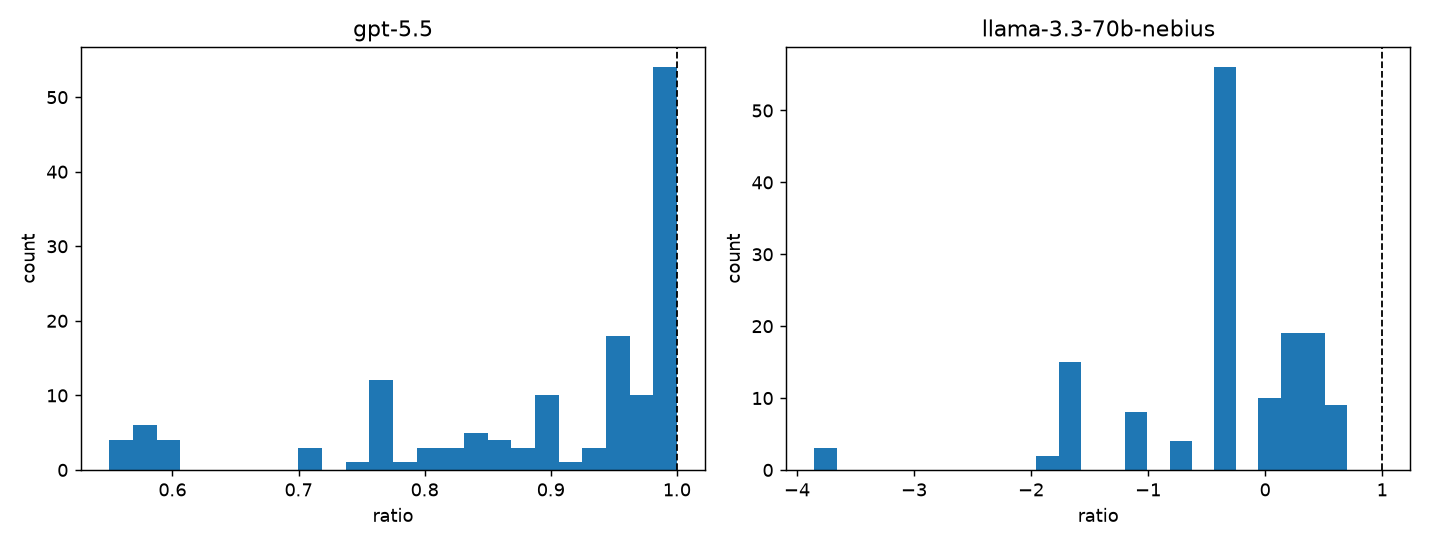
\includegraphics[width=0.85\textwidth]{results/fig3_ev_distributions.png}
\caption{EV-realization ratio distribution, evidence-bearing rounds, baseline arm, one panel per model. Shows the shape behind Table 1/2's percentiles: the weak model's mass straddling zero rather than one bad tail dragging the mean, against the frontier's near-ceiling concentration.}
\label{fig:3}
\end{figure}

\subsection{5.4\quad RQ3: Scaffold effectiveness and attribution}\label{rq3-scaffold-effectiveness-and-attribution}

The ablation runs the frozen five-condition matrix (baseline, +C1, +C2, +C1+C2, and the token-matched control) on both models at \texttt{N\ =\ 29} shared-seed episodes. Table 3 reports the three decision axes on evidence-bearing rounds (\texttt{round\ ≥\ 2}): estimation error (Oracle B: total-variation distance of the stated \texttt{V}-posterior from the correct one, lower is better), execution consistency (Oracle A: EV-realization ratio, higher is better), and composite decision quality (the action scored under the true model, higher is better). Two additional arms, \textbf{+C3a} and \textbf{+C3b}, are post-freeze follow-ups motivated by the mechanism this section diagnoses; they are introduced below and clearly marked as exploratory rather than part of the frozen matrix. Token and latency cost is reported in the same table family in §5.5, never separately.

\textbf{Table 3: Ablation across the three decision axes (evidence-bearing rounds, \texttt{N=29}; frontier / weak).} Each cell reports two point estimates, frontier then weak, separated by a slash.

{\def\LTcaptype{none} % do not increment counter
\begin{longtable}[]{@{}
  >{\raggedright\arraybackslash}p{(\linewidth - 6\tabcolsep) * \real{0.2941}}
  >{\raggedleft\arraybackslash}p{(\linewidth - 6\tabcolsep) * \real{0.2255}}
  >{\raggedleft\arraybackslash}p{(\linewidth - 6\tabcolsep) * \real{0.2451}}
  >{\raggedleft\arraybackslash}p{(\linewidth - 6\tabcolsep) * \real{0.2353}}@{}}
\toprule\noalign{}
\begin{minipage}[b]{\linewidth}\raggedright
Arm
\end{minipage} & \begin{minipage}[b]{\linewidth}\raggedleft
Belief TV distance ↓
\end{minipage} & \begin{minipage}[b]{\linewidth}\raggedleft
EV-realization ratio ↑
\end{minipage} & \begin{minipage}[b]{\linewidth}\raggedleft
Decision quality ↑
\end{minipage} \\
\midrule\noalign{}
\endhead
\bottomrule\noalign{}
\endlastfoot
Baseline & 0.063 / 0.135 & 0.89 / −0.37 & 0.93 / 0.61 \\
+ C1 (belief-state) & 0.088 / 0.187 & 0.88 / 0.34 & 0.93 / 0.69 \\
+ C2 (re-eval loop) & 0.060 / 0.246 & 0.90 / 0.34 & 0.93 / 0.07 \\
+ C1 + C2 (full scaffold) & 0.082 / 0.283 & 0.89 / 0.66 & 0.93 / 0.55 \\
Token-matched control & 0.052 / 0.117 & 0.91 / −0.16 & 0.93 / 0.71 \\
+ C3a (sufficient-statistic obs.) & 0.041 / 0.111 & 0.90 / −0.27 & 0.93 / 0.67 \\
+ C3b (de-duplicated carry) & 0.082 / 0.136 & 0.93 / −2.90 & 0.93 / 0.84 \\
\end{longtable}
}

The scaffold does not close the gap: it degrades the belief axis instead, and the belief-state carry (C1) turns out to be the single worst arm on the frontier. Against the token-matched control, the comparison that isolates structure from reasoning budget (§4.2), every scaffold arm has \emph{worse} beliefs, and the damage concentrates in C1: on the frontier its estimation error (TV 0.088) exceeds both the control (0.052) and the bare baseline (0.063), the contrast against the control excluding zero (+0.036, 95\% CI {[}+0.022, +0.051{]}), and its round-over-round directional agreement collapses (0.945 → 0.862; 0.738 for the full scaffold). Adding the re-evaluation loop does not recover it. This is a null result for the intervention as designed, and per the pre-registered null-result protection (§5) it is reported as the finding: a correctly-instrumented diagnosis shows the scaffold \emph{widens} the estimation gap rather than closing it.

The mechanism behind this is double-counting. C1 re-injects the agent's carried posterior while the frozen observation still shows the full raw flow history (F13) that posterior already summarizes; folding the same evidence in twice multiplies its likelihood in twice, which drives the stated posterior to be \emph{over-concentrated}. This predicts a signed, length-dependent signature that the symmetric TV distance cannot see: the concentration gap between the stated and correct posteriors should grow with round index and vanish at round 1. A zero-cost replay of the collected calls confirms exactly this: the per-round entropy gap regressed on round index is positive and excludes zero for the carry arms (frontier C1 +0.016/round, CI {[}+0.002, +0.031{]}; C1+C2 +0.026, CI {[}+0.010, +0.041{]}), flat for every no-carry arm, and ≈ 0 at round 1 where nothing has yet been carried. The weak model shows the same fingerprint, larger, and additionally over-concentrates under the re-evaluation loop (C2) alone. This is the failure mode Krishnamurthy et al. {[}13{]} isolate, that raw unsummarized history is the toxic ingredient even with chain-of-thought, reproduced here: C1 hands the model both a summary \emph{and} the raw history it duplicates.

\begin{figure}[htbp]
\centering
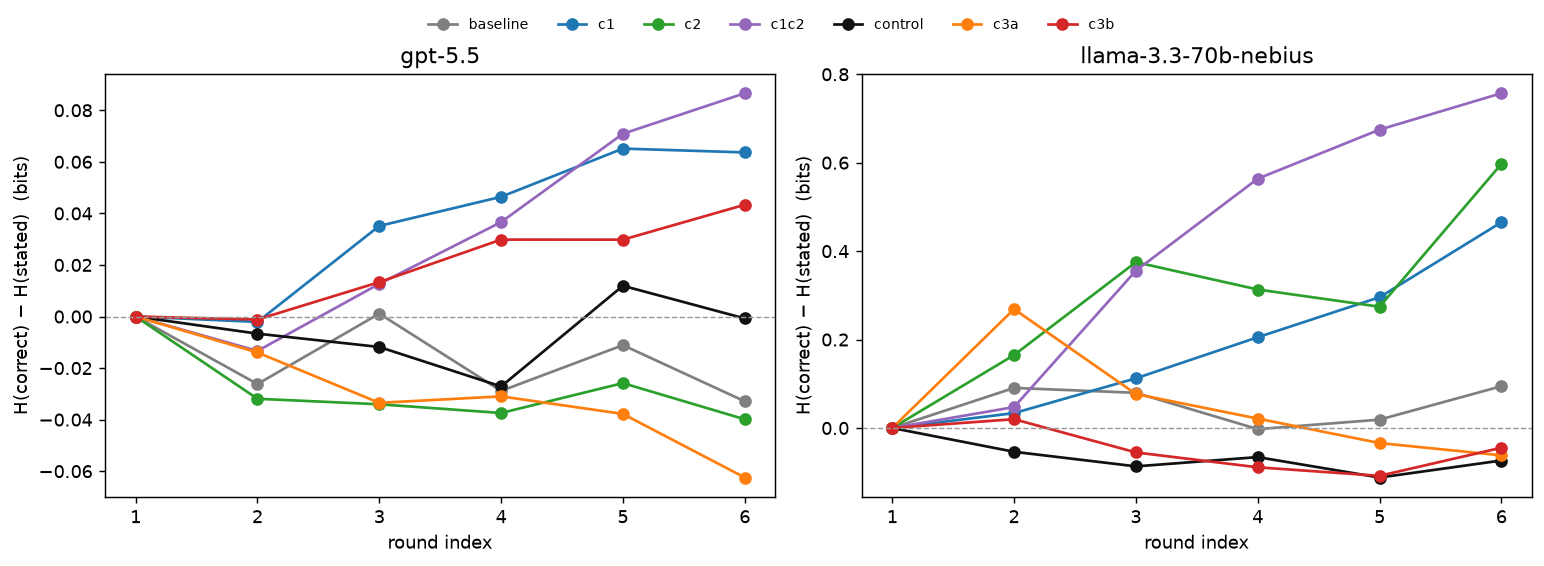
\includegraphics[width=0.85\textwidth]{results/belief_fingerprint_main.png}
\caption{mean entropy gap \texttt{H(correct) − H(stated)} vs. round index, one line per arm, one panel per model. The carry arms' upward slope against the flat no-carry arms is the over-concentration signature the CI numbers above summarize but don't show directly.}
\label{fig:4}
\end{figure}

The fingerprint implies a fix: present the flow as its sufficient statistic instead of the raw sequence. Because the correct \texttt{V}-posterior depends only on the counts of buy- vs.~sell-flow (flow direction is the only belief-relevant signal, since fills carry no information about \texttt{V} under the control-decoupling design (§3.1), and the update is order-independent), those counts are a \emph{lossless} summary of the belief-relevant history. C3a replaces the round-by-round observation with the cumulative buy/sell counts and drops the carry entirely; C3b instead keeps the carry but shows only the flow observed \emph{since} the recorded belief, de-duplicating the history while holding the carry constant. Both physically remove the redundant raw history through a C3-only observation renderer, an additive layer that leaves the frozen elicitation interface and the other five arms byte-identical. C3a attains the lowest estimation error of any arm on both models (frontier 0.041 vs.~control 0.052; weak 0.111 vs.~control 0.117) and \emph{reverses} the over-concentration fingerprint (its slope turns negative, excluding zero, on both models). C3b does not recover (frontier 0.082, on par with the full scaffold; weak 0.136, on par with baseline): de-duplicating the carry's history is not sufficient, which localizes the harm to the carry \emph{itself}, the model anchoring on its own prior stated belief, rather than to its duplication with the raw history.

The same fingerprint reappears on an independent frontier model and serving stack. As an Axis-2 robustness check (Post-Freeze Robustness Axes, optional and explicitly outside the frozen matrix), the full 7-arm ablation and the zero-cost fingerprint replay were repeated on GPT-5.6 Sol, a different, newer frontier model, run on Azure AI Foundry rather than the frozen matrix's OpenAI-direct GPT-5.5 (and a different serving stack again from the earlier OpenAI-direct GPT-5.6 probe, §3.5). The same signature reappears: the carry arms' entropy-gap slopes are positive and exclude zero (C1 +0.0648/round, CI {[}+0.0448, +0.0843{]}; C1+C2 +0.0354, CI {[}+0.0177, +0.0550{]}) against flat-to-negative reference arms (baseline ≈ 0, control −0.016), and C3a's slope again reverses sign (−0.0137, CI excludes zero) while C3b flattens it back toward zero: the same pre-registered gate criterion is confirmed, on a model that never appears in the frozen matrix. This is reported as a directional replication, not a second primary result: different model, different provider, not token-matched or determinism-frozen. Its only claim is that the double-counting mechanism is not an artifact of one model or one serving stack.

The composite decision-quality axis, however, shows the belief story does not transfer to decisions. Scoring each action under the true model, the bottom-line question of whether the decision was good in reality (§3.4), collapses the frontier differences entirely: all seven arms land at ≈ 0.93 (median 0.98), C3a's belief win included, and the paired C3a−C3b difference is −0.001 {[}−0.001, −0.000{]}. The frontier's \emph{actions} are near-optimal under truth and invariant to the scaffold, while what the scaffold moves is what the agent \emph{states} it believes, not what it does, and the residual \textasciitilde7\% decision gap is closed by no arm. On the weak model the axis instead exposes a dissociation: the best decisions come from C3b (0.84), not from the best-belief arm C3a (0.67). The weak model's decisive, committed framing under C3b yields better \emph{actual} trades on mediocre beliefs, while C3a's accurate beliefs do not convert into better actions. (The weak model's Oracle-A execution ratio is denominator-unstable here: its erratic stated beliefs push \texttt{EV(a*\ \textbar{}\ stated)} toward zero, producing the −2.90 tail, which is precisely why the true-model composite, with its stable denominator, is the reliable decision measure on the weak arm.)

Together, the two-oracle decomposition and the composite metric tell a sharper story than a single effectiveness number could. On the frontier, the scaffold's damage is confined to the stated-belief axis, while the real decisions were already good and stay good, so C3a repairs an axis that was not the binding constraint. On the weak model, belief accuracy and decision quality are \emph{decoupled}: the intervention that best fixes beliefs (C3a) is not the one that best fixes decisions (C3b), a knowing--doing dissociation the two-oracle instrument was built to expose but that only the composite adjudicates. The headline for RQ3 is therefore itself a decomposition: no arm closes the decision-quality gap on either model, the scaffold's belief-degradation is real but (on the frontier) cosmetic for decisions, and the belief and decision axes come apart on the weak model. Component attribution (C1 vs.~C2), the stated-vs-revealed inconsistencies of §3.3, and the C3a/C3b follow-ups all point the same way: in this instrument the decision-quality bottleneck is not where a belief-scaffolding intervention can reach it.

\clearpage

\subsection{5.5\quad RQ4: Efficiency and cost}\label{rq4-efficiency-and-cost}

Cost is logged per decision point from day one (§3.4), not reconstructed after the fact, so every cell below is an actual from the same \texttt{N=29} run as Table 3, priced at OpenAI's published GPT-5.5 rate (\$5.00/\$30.00 per M input/output tokens) {[}10{]} and Nebius Token Factory's published Llama-3.3-70B rate (\$0.13/\$0.40 per M) {[}20{]}.

\textbf{Table 4: Cost and efficiency per arm, relative to the no-scaffold baseline (\texttt{N=29}, 174 decisions/arm/model; frontier / weak).} Each cell reports two point estimates, frontier then weak, separated by a slash.

{\def\LTcaptype{none} % do not increment counter
\begin{longtable}[]{@{}
  >{\raggedright\arraybackslash}p{(\linewidth - 10\tabcolsep) * \real{0.1522}}
  >{\raggedleft\arraybackslash}p{(\linewidth - 10\tabcolsep) * \real{0.1413}}
  >{\raggedleft\arraybackslash}p{(\linewidth - 10\tabcolsep) * \real{0.2174}}
  >{\raggedleft\arraybackslash}p{(\linewidth - 10\tabcolsep) * \real{0.1196}}
  >{\raggedleft\arraybackslash}p{(\linewidth - 10\tabcolsep) * \real{0.1522}}
  >{\raggedleft\arraybackslash}p{(\linewidth - 10\tabcolsep) * \real{0.2174}}@{}}
\toprule\noalign{}
\begin{minipage}[b]{\linewidth}\raggedright
Arm
\end{minipage} & \begin{minipage}[b]{\linewidth}\raggedleft
Δ tokens/round ↓
\end{minipage} & \begin{minipage}[b]{\linewidth}\raggedleft
\$ total, N=29 (standard rate) ↓
\end{minipage} & \begin{minipage}[b]{\linewidth}\raggedleft
Latency ↓
\end{minipage} & \begin{minipage}[b]{\linewidth}\raggedleft
Δ decision quality ↑
\end{minipage} & \begin{minipage}[b]{\linewidth}\raggedleft
Quality per 1K extra tokens (weak only) ↑
\end{minipage} \\
\midrule\noalign{}
\endhead
\bottomrule\noalign{}
\endlastfoot
Baseline & n/a / n/a & \$1.15 / \$0.024 & 1.97s / 3.43s & n/a / n/a & n/a \\
+ C1 & +216 / +220 & \$1.34 / \$0.030 & 1.86s / 3.43s & 0.000 / +0.076 & 0.35 \\
+ C2 & +1515 / +1417 & \$2.70 / \$0.059 & 3.16s / 6.59s & 0.000 / −0.538 & negative \\
+ C1+C2 & +1947 / +1852 & \$3.08 / \$0.069 & 3.17s / 6.01s & 0.000 / −0.066 & negative \\
Token-matched control & +1871 / +2503 & \$4.48 / \$0.115 & 8.35s / 35.5s & 0.000 / +0.097 & 0.04 \\
+ C3a & −46 / −45 & \$1.12 / \$0.023 & 1.65s / 2.79s & −0.001 / +0.056 & free (cost-negative) \\
+ C3b & +195 / +197 & \$1.33 / \$0.029 & 1.62s / 2.32s & 0.000 / +0.224 & 1.14 \\
\end{longtable}
}

On the frontier, cost buys nothing: every scaffold arm spends more tokens for a decision-quality delta of ≈ 0.000. Each of the five arms was measured independently and happens to round to 0.000 at three decimals; §5.4 gives the unrounded frontier composite (all seven arms ≈ 0.93, paired C3a−C3b difference −0.001 {[}−0.001, −0.000{]}). The token-matched control is the extreme case: 2.8× the baseline's tokens per round, 4.2× its latency, and 3.9× its dollar cost at standard rates (\$4.48 vs.~\$1.15, the dollar ratio outrunning the token ratio because the control's overhead is almost entirely in the 6×-costlier output tokens, §4.2), for a decision-quality change indistinguishable from zero (§5.4). Every frontier ``efficiency'' number in this table is therefore a pure overhead number, since there is no numerator to put over it.

On the weak model, the cost story reproduces §5.4's dissociation: the intervention that pays for itself is not the one with the largest budget. C3a is cost-\emph{negative}: it removes the raw round-by-round history in favor of a fixed-size count summary, so both the frontier and weak arms spend fewer tokens than the baseline (−46 / −45 per round) while still improving weak-model decision quality (+0.056); its belief-axis win (§5.4) is, on this evidence, free. C3b spends only +197 tokens/round, a \textasciitilde21\% overhead, for the largest decision-quality gain in the study (+0.224), yielding 1.14 quality-points per 1K extra tokens, an order of magnitude more efficient than the token-matched control's 0.04. C2 and C1+C2 spend the \emph{most} tokens of any arm after the control (+1417 and +1852/round) and return \emph{negative} decision quality: the single clearest case in the matrix of cost bought no benefit, or actively subtracted one. The weak-model control additionally posts 27/174 invalid structured responses (§5.1) at 35.5s mean latency per round, a reliability and latency cost this table's dollar column does not capture, and one more reason C3-family arms (0/174 invalid on both models, sub-3s latency) are the practical choice if either were to be deployed.

Improvement per unit cost, not improvement alone, is the relevant comparison, and that framing changes the ranking from §5.4: C1+C2 (the ``full scaffold'') is the most expensive belief-carry arm and one of the worst performers on both axes it is supposed to help, while the two cheapest interventions in the entire matrix, C3a and C3b, both single-pass, both under the baseline's own token count on the frontier, are the only arms with an unambiguous, cost-justified win on the weak model. Cost efficiency does not rescue C1/C2's null result, and by this measure the null result looks worse, not better.

\begin{figure}[htbp]
\centering
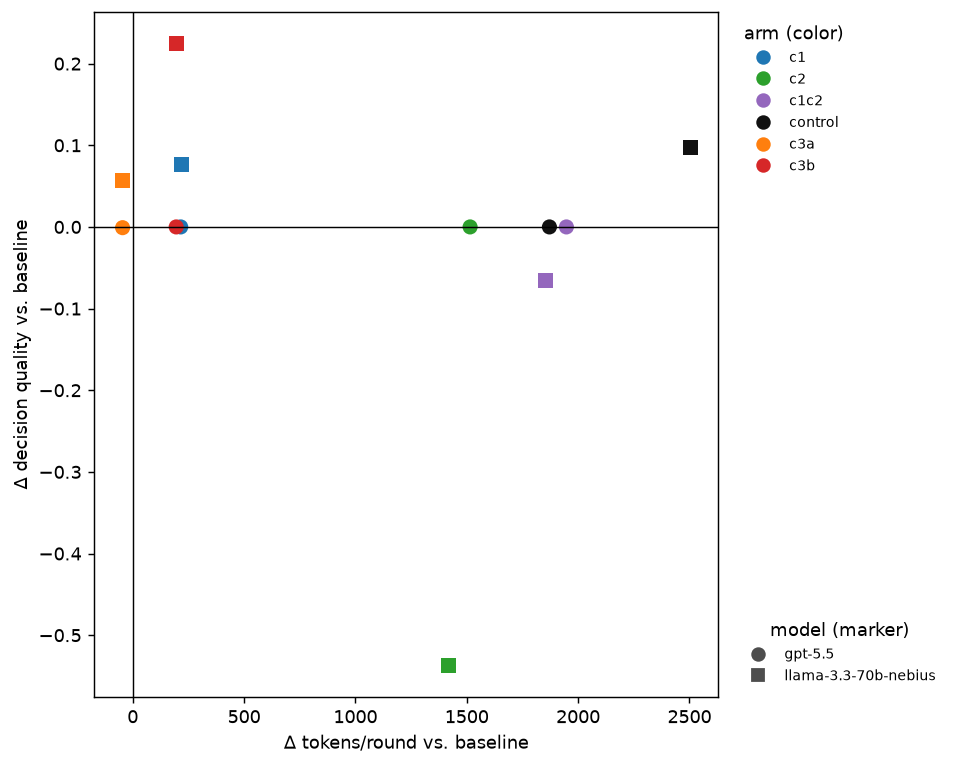
\includegraphics[width=0.85\textwidth]{results/fig5_cost_per_ev.png}
\caption{Δ tokens/round vs. Δ decision quality, one point per arm/model, relative to that model's baseline. Makes the quadrant pattern in Table 4 legible at a glance: C3a/C3b in the cheap-and-effective quadrant, C1+C2/control in the expensive-and-not quadrant.}
\label{fig:5}
\end{figure}
\FloatBarrier

\subsection{5.6\quad RQ5: Does native reasoning substitute for the scaffold? (secondary, directional)}\label{rq5-does-native-reasoning-substitute-for-the-scaffold-secondary-directional}

This question is secondary and directional, not part of the frozen matrix: it runs on a different model (GPT-5.6 Sol, Azure AI Foundry, not the frozen GPT-5.5), at \texttt{temperature=1} with no dated snapshot pin (\texttt{system\_fingerprint} is not populated on this deployment), under hidden-trace reasoning (\texttt{reasoning\_effort=\textquotesingle{}medium\textquotesingle{}}) rather than the same-pass elicitation the rest of §5 relies on. These caveats travel with every number below.

\textbf{Table E1: Reasoning-OFF vs.~reasoning-ON, all six arms, GPT-5.6 Sol (Azure), \texttt{N=29} (evidence-bearing rounds where noted; full-round ratios/regret shown to match Table D1).}

{\def\LTcaptype{none} % do not increment counter
\begin{longtable}[]{@{}
  >{\raggedright\arraybackslash}p{(\linewidth - 10\tabcolsep) * \real{0.1795}}
  >{\centering\arraybackslash}p{(\linewidth - 10\tabcolsep) * \real{0.0769}}
  >{\raggedleft\arraybackslash}p{(\linewidth - 10\tabcolsep) * \real{0.2051}}
  >{\raggedleft\arraybackslash}p{(\linewidth - 10\tabcolsep) * \real{0.1795}}
  >{\raggedleft\arraybackslash}p{(\linewidth - 10\tabcolsep) * \real{0.1538}}
  >{\raggedleft\arraybackslash}p{(\linewidth - 10\tabcolsep) * \real{0.2051}}@{}}
\toprule\noalign{}
\begin{minipage}[b]{\linewidth}\raggedright
Arm
\end{minipage} & \begin{minipage}[b]{\linewidth}\centering
Regime
\end{minipage} & \begin{minipage}[b]{\linewidth}\raggedleft
EV-realization ratio ↑
\end{minipage} & \begin{minipage}[b]{\linewidth}\raggedleft
Median ratio ↑
\end{minipage} & \begin{minipage}[b]{\linewidth}\raggedleft
EV regret ↓
\end{minipage} & \begin{minipage}[b]{\linewidth}\raggedleft
Directional agreement ↑
\end{minipage} \\
\midrule\noalign{}
\endhead
\bottomrule\noalign{}
\endlastfoot
Baseline & OFF & 0.864 & 0.833 & 0.170 & 0.821 \\
Baseline & ON & 0.838 & 0.894 & 0.176 & 0.993 \\
+ C1 & OFF & 0.845 & 0.912 & 0.270 & 0.924 \\
+ C1 & ON & 0.819 & 0.860 & 0.209 & 0.993 \\
+ C2 & OFF & 0.901 & 0.919 & 0.127 & 0.924 \\
+ C2 & ON & 0.797 & 0.860 & 0.216 & 1.000 \\
+ C1 + C2 & OFF & 0.868 & 0.912 & 0.231 & 0.572 \\
+ C1 + C2 & ON & 0.807 & 0.875 & 0.253 & 1.000 \\
+ C3a & OFF & 0.905 & 0.919 & 0.114 & 0.966 \\
+ C3a & ON & 0.777 & 0.895 & 0.235 & 0.993 \\
+ C3b & OFF & 0.853 & 0.842 & 0.214 & 1.000 \\
+ C3b & ON & 0.814 & 0.912 & 0.194 & 1.000 \\
\end{longtable}
}

OFF rows reuse Table D1; ON rows are new. All 1,044 ON-regime decision points across the six arms are valid, 0 invalid, 0 transport errors.

Reasoning-on does not help EV-realization on any arm: it is flat-to-negative across the board, and the drop is largest on the arm that needed it least. Every arm's mean ratio falls under reasoning-on; C3a, the best off-reasoning performer in the entire study (Table D1, 0.905), drops the most, to 0.777. Native reasoning does not substitute for structure on this task, on any scaffold variant tested, on this model.

The double-counting directional-agreement collapse (Table D1, C1+C2: 0.572) is absent under reasoning-on, but this should be read cautiously rather than as ``reasoning fixes it.'' Off-reasoning, the collapse is specific to the C1+C2 combination, not belief-carry alone (C1 sits at 0.924 off-reasoning, close to the token-matched control's 0.938, an important correction to the working hypothesis that running C1 in isolation under reasoning-on was designed to catch). Under reasoning-on, both C1 (0.993) and C1+C2 (1.000) sit at or near ceiling, same as every other arm. Two reasons this is not read as a repair:

\begin{enumerate}
\def\labelenumi{\arabic{enumi}.}
\tightlist
\item
  Hidden reasoning is a different measurement regime, not the same construct: \texttt{directional\_agreement} under reasoning-on scores an \emph{after-the-hidden-reasoning} stated belief against the action, so a high rate here may reflect the visible belief field being retrofit to an already-decided action (a caveat pre-registered for this axis), not that the action correctly followed the belief.
\item
  EV-realization moves the wrong way for this to count as a genuine fix: if reasoning-on actually resolved the double-counting defect, EV-realization on C1+C2 should improve, not fall (0.868 → 0.807). The more defensible reading is that the different measurement regime suppresses the \emph{diagnostic signal} this metric is built to detect, rather than resolving the underlying execution problem.
\end{enumerate}

Taken together, native reasoning is not a substitute for the external scaffold on this task: it does not improve EV-realization on any arm, and its one apparent repair (the C1+C2 directional-agreement collapse) does not survive cross-checking against EV-realization, which moves the wrong way for that reading to hold. This closes the obvious reviewer question, ``why not just use a reasoning model instead of the scaffold?'', with a directional but consistent negative answer. See Appendix E for provenance and cost.

\section{6\quad Discussion and Limitations}\label{discussion-and-limitations}

Every limitation below was identified during instrument design, before any result existed, rather than discovered after the fact: the instrument was designed around these risks, not surprised by them.

\begin{itemize}
\tightlist
\item
  Several nodes in the action grid have EV-optimal actions separated by a small margin, so an argmax-label accuracy metric would be dominated by noise near the flip. Every headline result in §5 is reported on continuous metrics (EV-realization ratio, EV regret), never on whether the agent's action label matched the argmax exactly. This is why the oracle unit tests assert the full 9-action EV vector rather than just the argmax.
\item
  The uniform-prior node's adverse-selection coefficient is sensitive to the informed-arrival share as it approaches the boundary, creating a knife-edge degeneracy as that share goes to zero. The logged omega distribution across collected episodes was checked to stay away from that degenerate region, so the reported EV-realization ratios are not artifacts of an unstable oracle near a knife-edge.
\item
  With only six rounds per episode, the sub-metric that infers the counterparty arrival mix from observed flow has few data points to work with and is correspondingly low-power by design, so conclusions in §5 rely on the belief-consistency (TV distance, directional agreement) and EV metrics, which do not depend on that inference, rather than on arrival-mix estimates themselves.
\item
  Decisions within an episode are not independent: intra-episode ICC is 0.211 on evidence-bearing rounds (GPT-5.5 baseline, \texttt{H=6}), giving a design effect of ≈1.84 at the five evidence-bearing decisions per episode. \texttt{N=29} episodes were chosen, not a smaller pilot size, specifically so that the resulting \textasciitilde2.7×29 effective independent decisions keep power adequate under this correlation rather than assuming naive independence across all 174 raw decision points.
\item
  The pre-freeze determinism check (§3.5, mechanism and per-decision detail) found GPT-5.5 is not perfectly deterministic at temperature 0: a small fraction of identical prompts produce a different action (``prior-collapse'' flips). This was accepted, not silently absorbed: serving noise was estimated to contribute only ≈0.006--0.008 to the aggregate standard error, under 6\% of the \textasciitilde0.135 evidence-bearing headroom the reported effects rely on, and that ``washes out'' argument only holds at the N≈29--57 range actually used, so it does not license extrapolating the frontier results to a smaller pilot-sized run.
\item
  The environment is a minimal repeated-pricing game rather than an OS-level or tool-use task, a trade §2.2 argues was necessary rather than incidental: no exact oracle exists for richer harnesses, and an approximate oracle would make execution error and oracle error indistinguishable. The instrument measures a real failure class with an exact ground truth in a small setting. Whether the same estimation/execution decomposition holds in richer settings like the ones ActPlane targets, where only approximate or compliance-based oracles are available, is the natural next step, not something this design can answer directly.
\item
  All main-matrix results (§5.2--5.5) are collected with \texttt{reasoning\_effort=\textquotesingle{}none\textquotesingle{}} as the primary operating point, for determinism and clean token accounting. Appendix E's reasoning-on probe is a genuinely different measurement regime: the model's hidden reasoning trace is not observed, only its effect on the same-pass elicited belief and action, and its finding (reasoning-on is flat-to-negative for EV-realization on every arm) is reported as a distinct, secondary axis, not folded into the main reasoning-off conclusions.
\item
  The scaffold-effect findings (§5.4) are demonstrated on one weak model, one frontier model, and, as a directional robustness check only (Appendix D), one additional frontier deployment (GPT-5.6 Sol on Azure), so their generalization is limited accordingly. The double-counting mechanism replicates on that second deployment, which is evidence against a single-model or single-serving-stack artifact, but three models sharing two architecture families is not a claim that the mechanism generalizes across all scaffold designs or all model families, only a claim about \emph{this} scaffold's specific failure mode, diagnosed with an instrument built to generalize even where this particular finding may not.
\item
  One untried mitigation is a directive that audits action-belief consistency directly. Every scaffold component tested here (C1, C2, C3a/C3b) and the reasoning-on/off axis (§5.6) operate on the belief layer, improving belief accuracy or reducing staleness, and none closes the frontier's execution gap. One further mechanism was not attempted: a directive asking the agent, at the execution step itself, whether the action it chose follows from the EV-implications of the belief it just stated, rather than auditing the belief's accuracy. This is the one lever in this design space that targets execution directly instead of the belief that precedes it. It was not implemented because the frontier's divergence from Oracle A is systematically conservative, narrower or smaller than the belief-optimal action, never the reverse under this prompt (§5.3, though §4.3 finds the direction does not hold under every paraphrase tested), so a directive tuned to catch this specific pattern risks correcting exactly the one bias this study measures rather than a general failure mode. Distinguishing ``fixed a real execution failure'' from ``trained away this study's own measured bias'' would require a separate validation study outside this project's scope. Recorded here as a future-work candidate, not as new scope for this project.
\end{itemize}

\section{7\quad Related Work}\label{related-work}

This work sits at the intersection of agent-harness reliability, LLM decision-making under uncertainty, and test-time scaffolding, placed here, late, in the systems-conference convention of engaging directly-adjacent work first before broadening.

In agent-harness reliability, ActPlane {[}28{]} documents the same knowing--doing gap this project measures (§2.1), but it has no ground-truth optimal action to compare against, so a violation is detected, not decomposed into a wrong belief versus a right belief the agent failed to act on. This project's differentiator is a same-pass-elicited belief plus an exact EV oracle, which together separate \emph{estimation error} (the belief was wrong) from \emph{execution error} (the belief was fine, the action didn't follow): the ``knew but didn't act'' failure that a compliance rate cannot see.

A second line of work evaluates LLM agents in sequential decision-making and games, which is well-established rather than novel: behavioural game theory has been applied to LLMs playing finitely repeated 2×2 games against scripted strategies and against humans {[}1{]}, generalized into game-theoretic benchmarks spanning complete/incomplete-information and deterministic/probabilistic tasks {[}8{]}, and extended to interactive environments more broadly {[}18{]}. Market and trading environments in particular are a recognized testbed, from portfolio-level benchmarks {[}16{]} to order-level simulators modeling latency, slippage, and book microstructure {[}22{]}. The repeated-pricing game here sits in the incomplete-information, dynamic, probabilistic quadrant of that taxonomy, the quadrant where LLMs are reported to be \emph{most} competitive {[}8{]}, which makes it a demanding rather than a convenient place to look for a gap. What this literature almost uniformly lacks is an exact ground-truth optimal action to score a decision against, and the evaluation currency reflects it: realized payoff and cooperation rates {[}1{]}, competitive win rate against another model {[}8{]}, end-to-end task success {[}18{]}, cumulative return and Sharpe ratio {[}16{]}. Each of these is an \emph{outcome} measure, terminal, aggregate, and counterfactual-free, so a failure can be observed but not attributed: none can say whether an agent held the wrong belief or held the right one and failed to act on it. Scoring an LLM against a \emph{normative} standard rather than against peers or humans is not itself unprecedented: GPT's choices have been graded for consistency with utility maximization and found largely rational {[}5{]}. But that check is a within-snapshot coherence test on static, one-shot decisions, where no belief evolves and therefore nothing can go stale or be mis-executed. The instructive near-exception is regret {[}23{]}, which \emph{is} optimality-referenced and which we do not overclaim against. But regret is measured against the best fixed action in hindsight and summed over an episode, so it necessarily \emph{aggregates} estimation and execution error rather than separating them, which is precisely the decomposition this instrument is built to produce. Two further results bracket the contribution. Prior work has already named the knowing--doing gap and measured it in bandits and Tic-tac-toe {[}24{]}, so the phenomenon studied here is not new, but that work closes the gap by RL fine-tuning on self-generated rationales, where this project's intervention is a no-training scaffold, and it scores actions against the \emph{true} optimum rather than against the agent's own stated belief, which collapses the very distinction the two-oracle design preserves. Separately, LLMs in bandit environments have been found to explore adequately in exactly one configuration: chain-of-thought \emph{plus an externally summarized interaction history presented as sufficient statistics}, with raw unsummarized history failing even with chain-of-thought {[}13{]}. That result both motivates the externalized belief-state component (§4.1, C1) and independently supports the token-matched control (§4.2), since its own decisive contrast holds reasoning tokens fixed and varies only the structure.

The instrument's dependence on a \emph{stated} belief also connects it to a literature on belief elicitation and calibration, on whether such statements mean anything in the first place. Models can emit a numeric confidence as text that maps to calibrated probabilities and that tracks their own uncertainty rather than imitating human confidence conventions {[}17{]}, and they carry self-knowledge recoverable by direct self-evaluation, though only, in the authors' own phrasing, ``when provided in the right format'' {[}12{]}. That caveat is load-bearing, because the elicitation protocol turns out to be a measurement instrument in its own right, not a formatting detail: for RLHF-tuned models, verbalized confidences emitted as output tokens are \emph{better} calibrated than the model's own conditional probabilities, cutting expected calibration error by roughly half {[}25{]}, and elicitation decomposes into prompting, sampling, and aggregation components each of which moves the measured calibration {[}27{]}. Two consequences follow for this design. First, eliciting the belief in tokens rather than reading it from logits is, on this evidence, the better-calibrated channel and not a concession forced by API access. Second, verbalized confidence is systematically \emph{overconfident} {[}27{]}, which sharpens the interpretation of the frontier finding (§5.3): an agent whose stated posterior is too narrow should quote \emph{tighter} and size \emph{up} relative to what the true model warrants, so a measured execution error in the direction of unjustified \emph{conservatism} runs against this prior rather than being predicted by it. Scored directly against a zero-cost replay of the collected decisions, rather than inferred from the ratio's shape, the frontier's divergence from its own belief-optimal action is systematically conservative, while the weak model's is systematically the opposite (§5.2, §5.3). This is a stronger claim than the ratio shape alone supports: it is exactly the direction the overconfidence prior predicts \emph{against} on the frontier, while failing to predict either the sign or the axis-dependence of the weak model's divergence. That said, the prompt-sensitivity check (§4.3) qualifies how far this generalizes: the conservative-direction pattern holds under one alternate surface form (Variant C, numbered rules) but not the other (Variant B, continuous prose, net aggressive on spread), so ``the frontier is conservative'' should be read as a finding about the baseline prompt and one of its two paraphrases, not as fully surface-form-invariant.

The stronger reason to elicit belief and action in a single forward pass is that stated reasoning produced \emph{separately} from an action is unreliable evidence about that action. Chain-of-thought explanations can systematically misrepresent the true cause of a model's output, rationalizing answers that were in fact driven by unmentioned features of the input {[}26{]}, and intervention studies show models vary widely in how much they actually condition on their own stated reasoning, with faithfulness \emph{decreasing} as models grow more capable {[}14{]}, a pointed prediction for the frontier arm (§5.3). A two-call protocol, act, then ask what you believed, is maximally exposed to exactly this post-hoc rationalization, which is what makes same-pass elicitation (§3.3) a validity requirement rather than an implementation convenience. The concern is concrete rather than hypothetical, since pointwise and joint querying have been shown to induce genuinely \emph{different} elicited beliefs, with downstream consequences for the resulting decisions {[}15{]}. The nearest neighbours to this project's thesis confirm the phenomenon while leaving the decomposition open. An ``action--belief gap'' has been documented directly: models bet against their own high-confidence predictions in a prediction market, fail to seek information when their stated confidence is low, and, critically, static calibration turns out to be an insufficient predictor of this dynamic consistency, with better-calibrated models sometimes \emph{less} consistent {[}21{]}. But that gap is measured by eliciting confidence in a static setting and comparing it to behaviour in a separate interactive one, which confounds ``the belief did not drive the action'' with ``the belief elicited in one context was not the belief held in the other'' (the confound same-pass elicitation exists to remove), and its consistency checks are directional rather than quantified against an exact optimum. Running the same split on self-efficacy estimates yields the opposite verdict: decisions were approximately rational \emph{given} the model's stated probabilities of success, and the miscalibration of those probabilities did the damage {[}4{]}. That prior work lands cleanly on estimation error, where this project's weak-model baseline (§5.2) finds both channels severely broken at once: beliefs barely better than chance (directional agreement 0.524) and execution that loses value on a majority of decisions (mean ratio −0.369). This is not a contradiction to be smoothed over: their elicited object is a scalar self-assessment and their rationality check is a coarse pursue/don't-pursue threshold, whereas Oracle A conditions on a belief about the \emph{environment} and computes an exact expected value over a nine-action grid, which resolves systematic action distortions that a binary threshold would score as approximately rational.

On test-time scaffolding and chain-of-thought controls, the token-matched unstructured control (§4.2) sits in the same lineage as chain-of-thought and other test-time-compute scaffolding work: the finding this project reports is specifically the \emph{structure's} effect over and above whatever benefit additional reasoning tokens already provide, which is what makes the token-matched control, not the bare baseline, the correct comparison arm.

\section{8\quad Conclusion}\label{conclusion}

This project built a two-oracle instrument, an exact EV oracle and an exact posterior oracle, paired with same-pass belief elicitation, small enough to admit closed-form ground truth, and used it to decompose LLM sequential-decision failure into estimation error and execution error rather than reporting a single blended gap. The finding is that both channels matter and neither subsumes the other: a weak model (Llama 3.3 70B) is severely broken on both axes (directional agreement barely above chance, mean EV-realization ratio negative), while a frontier model (GPT-5.5) has largely correct beliefs but still forfeits value on two-thirds of its decisions relative to its own stated reasoning. Capability relocates the gap from estimation to execution rather than closing it. Testing a no-training scaffold against this instrument, rather than against a proxy metric, produced a result a coarser measure would have missed entirely: the scaffold's belief-carry component \emph{widens} the estimation-error axis it was built to fix, via a diagnosable double-counting mechanism, replicated on an independent frontier model. A follow-up sufficient-statistic fix repairs that axis at negative token cost, yet a true-model decision-quality metric shows this belief repair is largely cosmetic on the frontier and dissociates from decision quality on the weak model, where a cheaper, different intervention delivers the study's largest and most cost-efficient gain instead. Reported jointly with token, latency, and dollar cost throughout (never effectiveness alone), the result is that a plausible and cheap intervention can move the axis it targets in the wrong direction while leaving the decisions that matter unchanged: a distinction invisible to any harness-reliability metric that checks only whether an action was correct, not whether it followed from what the agent said it believed. For agent-harness reliability more broadly, the implication is that ``the agent's stated reasoning looks right'' and ``the agent's scaffold is working'' are separate empirical claims, and treating them as one is exactly the blind spot this instrument was built to close.

\section{Acknowledgments}\label{acknowledgments}

I thank Prof.~Wei Wang, Department of Computer Science and Engineering, HKUST, for advising this project.

\section{A\quad Frozen base prompt}\label{a-frozen-base-prompt}

Variant A is the primary prompt, used in every matrix row. Variants B and C are information-equivalent by construction: each asserts the identical fact set F1--F15 below and nothing else, differing only in surface form, and exist solely for the §4.3 prompt-sensitivity check.

\textbf{F1--F15 (the information-equivalence contract):}

\begin{itemize}
\tightlist
\item
  \textbf{F1} Role: market maker, single asset, multi-round episode.
\item
  \textbf{F2} \texttt{V\ ∈\ \{10,\ 15,\ 20\}}, drawn uniformly at random at episode start, fixed all episode, revealed only after the final round.
\item
  \textbf{F3} Fixed number of rounds; each round's message shows the current round number and the total.
\item
  \textbf{F4} Exactly one counterparty arrives per round.
\item
  \textbf{F5} Two types, never revealed. Informed knows \texttt{V}: buys if \texttt{V\ =\ 20}, sells if \texttt{V\ =\ 10}, 50/50 if \texttt{V\ =\ 15}. Uninformed: 50/50 regardless of \texttt{V}.
\item
  \textbf{F6} Types drawn independently per arrival; the informed share is fixed throughout and not disclosed.
\item
  \textbf{F7} Buy/sell direction does not depend on the quote; only trade completion does.
\item
  \textbf{F8} Quotes symmetric around \texttt{m\ =\ 10*v10\ +\ 15*v15\ +\ 20*v20} computed from the stated \texttt{belief\_v}; tight/medium/wide = bid/ask at \texttt{m\ ∓\ 1}, \texttt{m\ ∓\ 2}, \texttt{m\ ∓\ 3}.
\item
  \textbf{F9} Size ∈ \{1, 2, 3\}; a completed trade is for the full size.
\item
  \textbf{F10} Completion is probabilistic; probability falls as spread widens and size grows; exact probabilities not disclosed.
\item
  \textbf{F11} Payoff \texttt{size*(ask\ −\ V)} on buys, \texttt{size*(V\ −\ bid)} on sells; settled at episode end when \texttt{V} is revealed.
\item
  \textbf{F12} Qualitative selection: completed trades with informed counterparties tend to be losses; with uninformed, profits.
\item
  \textbf{F13} Observation history per prior round: own (spread, size); flow direction (observed whether or not the trade completed); fill outcome; or, if that round's elicitation was invalid after retries, the fixed neutral notice that no valid quote was produced, with flow direction still disclosed.
\item
  \textbf{F14} Objective: maximize total profit over the episode.
\item
  \textbf{F15} Output contract: a single JSON object and nothing else; fields in order \texttt{belief\_v\{v10,\ v15,\ v20\}} (non-negative, sum to 1), \texttt{belief\_informed\_share} ∈ {[}0, 1{]} (proportion of arrivals that are informed), \texttt{action\{spread\ ∈\ tight\textbar{}medium\textbar{}wide,\ size\ ∈\ 1\textbar{}2\textbar{}3\}}; beliefs stated before the action.
\end{itemize}

\textbf{Variant A: primary (headed spec), verbatim:}

\begin{Shaded}
\begin{Highlighting}[]
\NormalTok{You are a market maker in a multi{-}round trading game involving a single asset.}

\NormalTok{THE ASSET. The asset has a hidden true value V, which is 10, 15, or 20. At the start of the episode, V was drawn uniformly at random from these three values (each equally likely). V stays fixed for the entire episode and is revealed only after the final round. Each round\textquotesingle{}s message tells you the current round number and the total number of rounds in the episode.}

\NormalTok{COUNTERPARTIES. Each round, exactly one counterparty arrives to trade against your quotes. Every counterparty is one of two types, and you are never told which:}
\NormalTok{{-} Informed: knows V. Buys if V = 20, sells if V = 10, and is equally likely to buy or sell if V = 15.}
\NormalTok{{-} Uninformed: does not know V. Is equally likely to buy or sell, whatever V is.}
\NormalTok{Each arriving counterparty\textquotesingle{}s type is drawn independently, and the proportion of informed arrivals is the same throughout; that proportion is not disclosed to you. A counterparty\textquotesingle{}s choice to buy or sell does not depend on your quote; only whether the trade completes does.}

\NormalTok{YOUR QUOTES. Each round you choose a spread and a size. Your bid and ask are placed symmetrically around the midpoint m implied by the beliefs you state in the same response: m = 10*v10 + 15*v15 + 20*v20. A tight spread quotes bid m {-} 1 and ask m + 1; medium quotes m {-} 2 and m + 2; wide quotes m {-} 3 and m + 3. Size is 1, 2, or 3 units; a completed trade is always for your full quoted size.}

\NormalTok{TRADES AND PROFITS. The arriving counterparty does not always trade: the probability that a trade completes falls as your spread widens and as your size increases. The exact probabilities are not disclosed to you. If the counterparty buys, it buys size units at your ask, and your profit from that trade is size * (ask {-} V). If it sells, it sells size units at your bid, and your profit is size * (V {-} bid). Profits are settled at the end of the episode, when V is revealed. Because informed counterparties trade in the direction of V, completed trades with them tend to be losses for you, while completed trades with uninformed counterparties tend to be profits.}

\NormalTok{WHAT YOU OBSERVE. Each round\textquotesingle{}s message includes the full history of prior rounds: the spread and size you quoted, the direction of the counterparty\textquotesingle{}s flow (buy or sell {-} you observe this whether or not a trade completed), and whether your quote was filled.}

\NormalTok{OBJECTIVE. Maximize your total profit over the episode.}

\NormalTok{YOUR RESPONSE. Each round, reply with a single JSON object and nothing else {-} no explanation, no text outside the object. Fill in its fields in the order listed, stating your beliefs first and then choosing your action:}
\NormalTok{{-} "belief\_v": an object with keys "v10", "v15", "v20" {-} your current probability that V is 10, 15, or 20. Three non{-}negative numbers that sum to 1.}
\NormalTok{{-} "belief\_informed\_share": a number between 0 and 1 {-} your current belief about the proportion of arriving counterparties that are informed.}
\NormalTok{{-} "action": an object with "spread" (one of "tight", "medium", "wide") and "size" (1, 2, or 3).}

\NormalTok{Response format:}
\NormalTok{\{"belief\_v": \{"v10": \textless{}number\textgreater{}, "v15": \textless{}number\textgreater{}, "v20": \textless{}number\textgreater{}\}, "belief\_informed\_share": \textless{}number\textgreater{}, "action": \{"spread": "\textless{}tight|medium|wide\textgreater{}", "size": \textless{}1|2|3\textgreater{}\}\}}
\end{Highlighting}
\end{Shaded}

Variants B (continuous prose) and C (numbered rules) are omitted here to avoid duplicating \textasciitilde2 pages of near-identical text; both assert the identical F1--F15 fact set as Variant A and differ only in surface form.

\section{B\quad Oracle validation anchors}\label{b-oracle-validation-anchors}

All values are exact \texttt{Fraction} arithmetic, verified by dedicated unit tests for both oracles, evaluated at stated \texttt{ω\ =\ 0.35} (\texttt{Fraction(7,\ 20)}), which for these anchors also equals the true \texttt{P(Informed)}.

\textbf{Node A: round-1 uniform prior.} \texttt{π\ =\ (1/3,\ 1/3,\ 1/3)}, \texttt{E{[}V{]}\ =\ 15}, \texttt{c\ =\ 10/3\ ≈\ 3.333}.

{\def\LTcaptype{none} % do not increment counter
\begin{longtable}[]{@{}lrr@{}}
\toprule\noalign{}
Action & EV (exact) & EV (decimal) \\
\midrule\noalign{}
\endhead
\bottomrule\noalign{}
\endlastfoot
tight, 1 & −19/120 & −0.1583 \\
tight, 2 & −43/100 & −0.4300 \\
tight, 3 & −73/80 & −0.9125 \\
medium, 1 & 77/150 & 0.5133 \\
medium, 2 & 3/5 & 0.6000 \\
medium, 3 & 13/50 & 0.2600 \\
wide, 1 (a*) & 103/150 & 0.6867 \\
wide, 2 & 37/60 & 0.6167 \\
wide, 3 & 3/8 & 0.3750 \\
\end{longtable}
}

\textbf{Node B: after three consecutive buys.} \texttt{π\ =\ (2197/29880,\ 200/747,\ 2187/3320)\ ≈\ (0.0735,\ 0.2678,\ 0.6588)}, \texttt{E{[}V{]}\ =\ 53563/2988\ ≈\ 17.926}, \texttt{c\ =\ 87003551/44640720\ ≈\ 1.949}.

{\def\LTcaptype{none} % do not increment counter
\begin{longtable}[]{@{}lrr@{}}
\toprule\noalign{}
Action & EV (exact) & EV (decimal) \\
\midrule\noalign{}
\endhead
\bottomrule\noalign{}
\endlastfoot
tight, 1 & 5392001317/17856288000 & 0.3020 \\
tight, 2 & 219308503/496008000 & 0.4421 \\
tight, 3 & 1922775431/5952096000 & 0.3230 \\
medium, 1 & 16520290871/17856288000 & 0.9252 \\
medium, 2 (a*) & 789717703/595209600 & 1.3268 \\
medium, 3 & 7171240219/5952096000 & 1.2048 \\
wide, 1 & 1198924303/1116018000 & 1.0743 \\
wide, 2 & 5780988001/4464072000 & 1.2950 \\
wide, 3 & 618594943/496008000 & 1.2471 \\
\end{longtable}
}

\textbf{Node C: one buy, one sell (cancelling evidence).} \texttt{π\ =\ (351/1102,\ 200/551,\ 351/1102)\ ≈\ (0.3186,\ 0.3630,\ 0.3186)}, \texttt{E{[}V{]}\ =\ 15} (exact, by symmetry), \texttt{c\ =\ 1755/551\ ≈\ 3.185}.

{\def\LTcaptype{none} % do not increment counter
\begin{longtable}[]{@{}lrr@{}}
\toprule\noalign{}
Action & EV (exact) & EV (decimal) \\
\midrule\noalign{}
\endhead
\bottomrule\noalign{}
\endlastfoot
tight, 1 & −253/2320 & −0.1091 \\
tight, 2 & −4637/13775 & −0.3366 \\
tight, 3 & −4299/5510 & −0.7802 \\
medium, 1 & 122857/220400 & 0.5574 \\
medium, 2 & 14939/22040 & 0.6778 \\
medium, 3 & 79599/220400 & 0.3612 \\
wide, 1 (a*) & 20061/27550 & 0.7282 \\
wide, 2 & 1899/2755 & 0.6893 \\
wide, 3 & 10323/22040 & 0.4684 \\
\end{longtable}
}

The argmax moves from \texttt{(wide,\ 1)} at diffuse belief (Nodes A, C) to \texttt{(medium,\ 2)} as belief concentrates in one direction (Node B): the belief-dependence the instrument requires, asserted directly in Oracle A's unit tests. Node C does not cross this flip; its role is purely to catch Bayes-update bugs under cancelling evidence, which Nodes A and B alone cannot test.

\textbf{Oracle B ceilings, by exact backward induction:}

{\def\LTcaptype{none} % do not increment counter
\begin{longtable}[]{@{}
  >{\raggedright\arraybackslash}p{(\linewidth - 4\tabcolsep) * \real{0.1250}}
  >{\raggedleft\arraybackslash}p{(\linewidth - 4\tabcolsep) * \real{0.2500}}
  >{\raggedright\arraybackslash}p{(\linewidth - 4\tabcolsep) * \real{0.6250}}@{}}
\toprule\noalign{}
\begin{minipage}[b]{\linewidth}\raggedright
Horizon
\end{minipage} & \begin{minipage}[b]{\linewidth}\raggedleft
Ceiling (exact)
\end{minipage} & \begin{minipage}[b]{\linewidth}\raggedright
Ceiling (decimal)
\end{minipage} \\
\midrule\noalign{}
\endhead
\bottomrule\noalign{}
\endlastfoot
\texttt{H=1} & 103/150 & 0.6867 (equals Node A's optimum exactly) \\
\texttt{H=2} & 6523/4500 & 1.4496 \\
\end{longtable}
}

\texttt{H=1}'s ceiling equaling Node A's Oracle A optimum exactly is itself a cross-oracle consistency check: at the very first round, before any observation exists, the two oracles must agree, since there is no estimation error yet to separate from execution error.

\section{C\quad Reproducibility}\label{c-reproducibility}

The repository, code, oracles, response caches, and every result and figure cited in this report are publicly available at \texttt{https://github.com/vmfan/akrasia}.

As described in §3.5, the simulator, both oracles, the elicitation interface, the metric code, and the frozen base prompt (Appendix A, Variant A) were fixed at the freeze gate. Everything reported in §5 for the seven main-matrix arms is computed against that frozen state; nothing in the frozen path was modified after it (§3). Post-freeze additions (belief-consistency, belief-fingerprint, decision-quality, PnL-vs-ceiling, conservatism, C3a/C3b) are pure additive analyses layered on top of frozen artifacts; none of them re-derive or replace a frozen component, and each is a separate module rather than an edit to frozen code.

A model name alone is not a reproducibility pin: provider, precision, snapshot, seed, and region together define the artifact actually queried. The two frozen-matrix models are pinned as follows:

{\def\LTcaptype{none} % do not increment counter
\begin{longtable}[]{@{}
  >{\raggedright\arraybackslash}p{(\linewidth - 4\tabcolsep) * \real{0.1731}}
  >{\raggedright\arraybackslash}p{(\linewidth - 4\tabcolsep) * \real{0.4135}}
  >{\raggedright\arraybackslash}p{(\linewidth - 4\tabcolsep) * \real{0.4135}}@{}}
\toprule\noalign{}
\begin{minipage}[b]{\linewidth}\raggedright
\end{minipage} & \begin{minipage}[b]{\linewidth}\raggedright
Frontier (GPT-5.5)
\end{minipage} & \begin{minipage}[b]{\linewidth}\raggedright
Weak (Llama 3.3 70B)
\end{minipage} \\
\midrule\noalign{}
\endhead
\bottomrule\noalign{}
\endlastfoot
Provider & OpenAI direct API & Nebius Token Factory \\
Model string / snapshot & \texttt{gpt-5.5-2026-04-23} (dated snapshot; no rolling alias) & \texttt{meta-llama/Llama-3.3-70B-Instruct} \\
Precision & (managed by provider; snapshot-pinned) & FP8: no serverless provider offers BF16 for this model (confirmed by verification testing) \\
Temperature & 0 & 0 \\
Reasoning effort & \texttt{reasoning\_effort=\textquotesingle{}none\textquotesingle{}} (explicit on every call) & n/a: no reasoning mode {[}19{]} \\
Determinism & Byte-identical actions on shallow prompts; known non-determinism on deep-history prompts (mechanism in §3.5, up to 6.66\% belief spread, 4/8 real-episode decisions over the 2\% tolerance); accepted per the determinism-floor argument (§6), not silently absorbed & Byte-identical on both shallow and deep cases at n=8 repeats; no determinism problem on this arm \\
Region / fingerprint & Standard OpenAI-direct \texttt{system\_fingerprint} logged per call & Nebius Token Factory; no per-region pin beyond the provider endpoint \\
\end{longtable}
}

Debug-only traffic (the HKUST API, used during early development before the frozen collection pipeline) is excluded from every reportable number: HKUST and Nebius were verified to diverge on identical prompts and seeds (HKUST mean −0.438 vs.~Nebius mean −0.543 on the same 8-episode check), so no HKUST-derived figure appears anywhere in §5 or the appendices.

All frozen-matrix and post-freeze-replay runs share one seed family: \texttt{BASE\_SEED\ =\ 7000}, with per-episode and per-fill RNG seeds derived deterministically from it (\texttt{EPISODE\_SEED\_BASE\ =\ 5000}, \texttt{FILL\_RNG\_SEED\_BASE\ =\ 6000}). The same \texttt{N=29} episode set, same seeds, is reused unchanged across all seven main-matrix arms, both post-freeze mechanism arms (C3a, C3b), and the zero-API replay analyses (belief-fingerprint, decision-quality, PnL-vs-ceiling, conservatism); replay is verified by asserting zero cache misses against the frozen response cache on every such run, which is the operational proof that a replay reproduced the original decisions exactly rather than re-deriving them.

Every model call is logged with model fingerprint/version string, seed, prompt hash, output hash, token counts, and latency from the first frozen run, never reconstructed after the fact. A silent provider redeploy is treated as equivalent to a \texttt{system\_fingerprint} change and would be visible in this log, not inferred from output drift.

Appendices D and E instead run on a directional, not frozen, deployment: the GPT-5.6 Sol robustness axis (Appendix D) and the reasoning-on/off cross (Appendix E) run on Azure AI Foundry, Tier 1, Japan East, pinned to a dated model version (\texttt{2026-07-09}) with auto-upgrade disabled. This deployment has two known, accepted reproducibility gaps not present on the frontier-matrix pin above: every call logs \texttt{snapshot\_mismatch:\ true} and \texttt{fingerprint:\ null} (no dated-snapshot / no-fingerprint guarantee on this Azure deployment), and the reasoning-on cells run at \texttt{temperature=1} rather than \texttt{0} (on this Azure AI Foundry deployment, reasoning mode rejects \texttt{temperature=0} {[}2{]}). Both appendices report their findings as directional evidence on this specific deployment, explicitly not as determinism-frozen or token-matched results, and are never folded into the frozen-matrix headline numbers in §5.

Given the freeze gate, the seeds, and the pins above, every number in Table 1--4 and the full ablation matrix is exactly reproducible by replaying the frozen cache (zero API cost) or, from scratch, by re-running the pinned frontier/weak endpoints at the stated seeds, modulo the frontier's own documented deep-history non-determinism, which is bounded and accepted, not eliminated. Appendix D/E numbers are reproducible only up to that deployment's own non-determinism and its unpinned fingerprint, and are reported with that caveat attached rather than presented as equivalent in rigor to the frozen matrix.

\section{D\quad Post-freeze robustness axis: GPT-5.6 Sol (Azure)}\label{d-post-freeze-robustness-axis-gpt-5.6-sol-azure}

GPT-5.6 Sol was evaluated once already, pre-freeze, on OpenAI direct: an \texttt{N=8}, \texttt{H=4} baseline-only, no-scaffold probe (0.913 mean EV-realization vs.~GPT-5.5's 0.929 at the same horizon) that fed the frontier-model decision and is not repeated here. Both figures predate the pre-freeze retune from \texttt{H=4} to \texttt{H=6} (§3.1) and are not directly comparable to this report's \texttt{H=6} headline numbers (e.g.~GPT-5.5's 0.893 in §5.3): the retune happened precisely because \texttt{H=4} left too little headroom below the ceiling, so a higher ratio at \texttt{H=4} reflects that shorter horizon, not model drift. This appendix reports the full ablation matrix on GPT-5.6 Sol as deployed on Azure AI Foundry (Tier 1, Japan East region, pinned model version \texttt{2026-07-09}, static API-key auth). The two GPT-5.6 datapoints, OpenAI-direct baseline and Azure full-matrix, sit on different serving stacks and are not merged or compared to each other; neither is compared to the frozen GPT-5.5 matrix as anything other than a qualitative reference point. Everything in this appendix is directional signal only: not determinism-frozen, not token-matched, not part of the frozen matrix, and not re-opening the frontier-model decision (§3.5).

On compatibility, before any scaffold-effectiveness data was collected, a 2-episode smoke test across all 7 registered arms (the frozen five plus the post-freeze +C3a/+C3b arms, §5.4) confirmed this deployment accepts \texttt{temperature=0}, a \texttt{seed}, and strict JSON-schema structured output (the same operating point the frozen matrix requires) with zero transport errors. The full \texttt{N=29} run reproduced this cleanly: 0 invalid responses across all 7 arms (1,740 decision points total).

Table D1 reports a different column set than Table 3: EV-realization ratio at both all-round and evidence-bearing scope, EV regret, belief TV distance, and directional agreement, rather than Table 3's belief TV distance / EV-realization ratio / decision quality. The composite decision-quality replay was not part of this directional axis's collection, so it has no entry here; the columns below are what this axis actually measured, not a reduced view of Table 3's.

\textbf{Table D1: GPT-5.6 Sol (Azure), full 7-arm ablation, \texttt{N=29} (evidence-bearing rounds, \texttt{round\ ≥\ 2}).}

{\def\LTcaptype{none} % do not increment counter
\begin{longtable}[]{@{}
  >{\raggedright\arraybackslash}p{(\linewidth - 10\tabcolsep) * \real{0.2553}}
  >{\raggedleft\arraybackslash}p{(\linewidth - 10\tabcolsep) * \real{0.1702}}
  >{\raggedleft\arraybackslash}p{(\linewidth - 10\tabcolsep) * \real{0.1702}}
  >{\raggedleft\arraybackslash}p{(\linewidth - 10\tabcolsep) * \real{0.1277}}
  >{\raggedleft\arraybackslash}p{(\linewidth - 10\tabcolsep) * \real{0.1277}}
  >{\raggedleft\arraybackslash}p{(\linewidth - 10\tabcolsep) * \real{0.1489}}@{}}
\toprule\noalign{}
\begin{minipage}[b]{\linewidth}\raggedright
Arm
\end{minipage} & \begin{minipage}[b]{\linewidth}\raggedleft
EV-realization ratio (all rounds) ↑
\end{minipage} & \begin{minipage}[b]{\linewidth}\raggedleft
EV-realization ratio (evidence-bearing) ↑
\end{minipage} & \begin{minipage}[b]{\linewidth}\raggedleft
EV regret ↓
\end{minipage} & \begin{minipage}[b]{\linewidth}\raggedleft
Belief TV distance ↓
\end{minipage} & \begin{minipage}[b]{\linewidth}\raggedleft
Directional agreement ↑
\end{minipage} \\
\midrule\noalign{}
\endhead
\bottomrule\noalign{}
\endlastfoot
Baseline & 0.864 & 0.836 & 0.170 & 0.067 & 0.821 \\
+ C1 & 0.845 & 0.814 & 0.270 & 0.081 & 0.924 \\
+ C2 & 0.901 & 0.881 & 0.127 & 0.055 & 0.924 \\
+ C1 + C2 & 0.868 & 0.841 & 0.231 & 0.080 & 0.572 \\
Token-matched control & 0.877 & 0.857 & 0.165 & 0.050 & 0.938 \\
+ C3a & 0.905 & 0.886 & 0.114 & 0.047 & 0.966 \\
+ C3b & 0.853 & 0.824 & 0.214 & 0.073 & 1.000 \\
\end{longtable}
}

The qualitative pattern matches the frozen GPT-5.5 finding of §5.4: C1 (belief-carry) is again the worst-or-near-worst scaffold arm on EV-realization, sitting below the bare baseline; C1+C2's directional agreement collapses sharply relative to the control (0.938 → 0.572, versus GPT-5.5's 0.945 → 0.738); and C3a is again the best arm on every column shown.

\textbf{Table D2: Belief double-counting fingerprint, GPT-5.6 Sol (Azure), zero-API cache replay of the Table D1 run.} Entropy-gap slope is \texttt{H(correct)\ −\ H(stated)} regressed on round index; positive and CI-excluding-zero is the over-concentration signature (§5.4).

{\def\LTcaptype{none} % do not increment counter
\begin{longtable}[]{@{}
  >{\raggedright\arraybackslash}p{(\linewidth - 4\tabcolsep) * \real{0.3429}}
  >{\raggedleft\arraybackslash}p{(\linewidth - 4\tabcolsep) * \real{0.2000}}
  >{\raggedright\arraybackslash}p{(\linewidth - 4\tabcolsep) * \real{0.4571}}@{}}
\toprule\noalign{}
\begin{minipage}[b]{\linewidth}\raggedright
Arm
\end{minipage} & \begin{minipage}[b]{\linewidth}\raggedleft
Slope / round
\end{minipage} & \begin{minipage}[b]{\linewidth}\raggedright
95\% CI
\end{minipage} \\
\midrule\noalign{}
\endhead
\bottomrule\noalign{}
\endlastfoot
Baseline & +0.0006 & {[}−0.0078, +0.0096{]} (crosses 0) \\
+ C1 & +0.0648 & {[}+0.0448, +0.0843{]} \\
+ C2 & −0.0018 & {[}−0.0168, +0.0155{]} (crosses 0) \\
+ C1 + C2 & +0.0354 & {[}+0.0177, +0.0550{]} \\
Token-matched control & −0.0161 & {[}−0.0287, −0.0022{]} \\
+ C3a & −0.0137 & {[}−0.0214, −0.0068{]} \\
+ C3b & +0.0011 & {[}−0.0150, +0.0177{]} (crosses 0) \\
\end{longtable}
}

The pre-registered gate criterion (§5.4), carry arms' slope CI excludes 0 and exceeds \texttt{max(baseline,\ control)}, is confirmed on this independent model and serving stack, matching the GPT-5.5/Llama result (§5.4). C3a's slope reversing sign and C3b's flattening back toward zero also reproduce, consistent with the belief-axis repair reported in §5.4.

\begin{figure}[htbp]
\centering
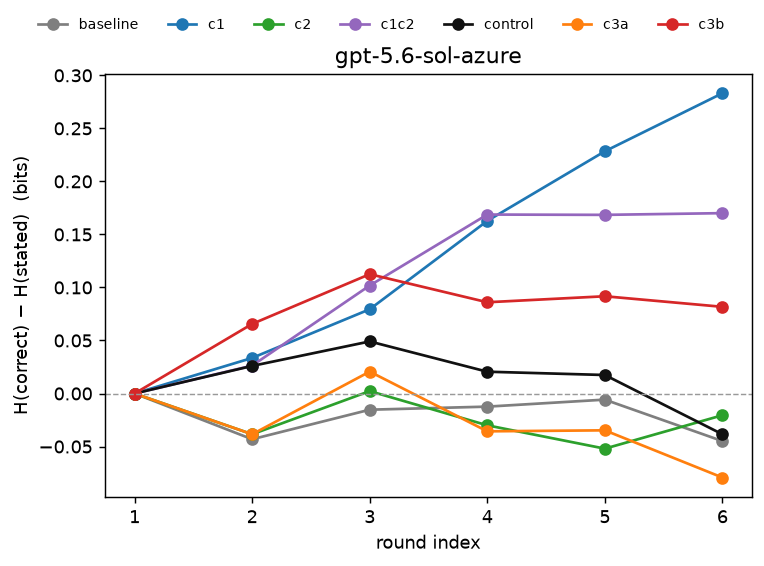
\includegraphics[width=0.85\textwidth]{results/belief_fingerprint_gpt56_azure.png}
\caption{same trajectory plot on this deployment's data. Included since it costs nothing beyond what produced Table D2 above, not because this directional appendix requires its own figure.}
\label{fig:4companion}
\end{figure}

This figure was re-rendered with the shared arm-color/legend styling used elsewhere in this report; the underlying numbers are unchanged from the original run.

On cost, this axis spent 2,117,450 input / 142,744 output tokens across all 7 arms at \texttt{N=29}, priced at GPT-5.6 Sol's published Azure AI Foundry rate (\$5.00/\$30.00 per M input/output tokens, identical to GPT-5.5's OpenAI-direct rate) {[}3{]}: ≈\$14.87.

\section{E\quad Axis 1: reasoning-on/off and the scaffold-mechanism cross (GPT-5.6 Sol, Azure)}\label{e-axis-1-reasoning-onoff-and-the-scaffold-mechanism-cross-gpt-5.6-sol-azure}

Axis 1 asks whether a model's own native reasoning subsumes the external scaffold: a full 6-arm cross (baseline, +C1, +C2, +C1+C2, +C3a, +C3b), each re-run with hidden reasoning (\texttt{reasoning\_effort=\textquotesingle{}medium\textquotesingle{}}, \texttt{temperature=1}, since this deployment's reasoning mode rejects \texttt{temperature=0} {[}2{]}) on GPT-5.6 Sol (Azure AI Foundry, Tier 1, Japan East), compared against the same arms' reasoning-off results (Appendix D). Formalizing the cross at the level of each individual scaffold mechanism, rather than the scaffold as a whole, asks whether native reasoning substitutes for, remediates, or complements each one separately. The token-matched control is excluded on structural grounds: a reasoning-on control column is uninterpretable, since hidden reasoning tokens void the token-matching that defines it.

Everything here is directional signal only: a different, non-same-pass measurement regime, not determinism-frozen, not token-matched, not part of the frozen matrix, and it does not reopen the frontier-model decision (§3.5). It also inherits the known reproducibility gap already documented for this deployment (Appendix D): no dated snapshot, \texttt{system\_fingerprint} not populated on any call. \texttt{reasoning\_effort=\textquotesingle{}medium\textquotesingle{}} + \texttt{temperature=1} acceptance was confirmed empirically by the first live call under this configuration (\texttt{valid:\ true}, no transport error, real reasoning-token counts), not assumed in advance.

This appendix covers provenance and cost for the reasoning-on/off cross; findings and Table E1 appear in §5.6 as RQ5 (secondary, directional).

This axis cost \$36.56 across the six arms. Cumulative GPT-5.6-Azure spend across the 7-arm ablation (Appendix D) and this axis comes to ≈\$51.43.

\section{References}\label{references}

\protect\phantomsection\label{refs}
\begin{CSLReferences}{0}{0}
\bibitem[\citeproctext]{ref-akata2023}
\CSLLeftMargin{{[}1{]} }%
\CSLRightInline{Akata, E., Schulz, L., Coda-Forno, J., Oh, S.J., Bethge, M. and Schulz, E. 2023. {Playing repeated games with large language models}. \emph{Nature Human Behaviour}. (2023). https://doi.org/\href{https://doi.org/10.1038/s41562-025-02172-y}{10.1038/s41562-025-02172-y}.}

\bibitem[\citeproctext]{ref-msazure2026reasoning}
\CSLLeftMargin{{[}2{]} }%
\CSLRightInline{{Azure OpenAI Reasoning Models}: 2026. \href{https://learn.microsoft.com/en-us/azure/foundry/openai/how-to/reasoning}{\emph{https://learn.microsoft.com/en-us/azure/foundry/openai/how-to/reasoning}}. Accessed 2026-07-21.}

\bibitem[\citeproctext]{ref-msazure2026openaipricing}
\CSLLeftMargin{{[}3{]} }%
\CSLRightInline{{Azure OpenAI Service Pricing}: 2026. \href{https://azure.microsoft.com/en-us/pricing/details/azure-openai/}{\emph{https://azure.microsoft.com/en-us/pricing/details/azure-openai/}}. Accessed 2026-07-22.}

\bibitem[\citeproctext]{ref-barkan2025}
\CSLLeftMargin{{[}4{]} }%
\CSLRightInline{Barkan, C.O., Black, S. and Sourbut, O. 2025. {Do Large Language Models Know What They Are Capable Of?} arXiv preprint arXiv:2512.24661. \url{https://arxiv.org/abs/2512.24661}.}

\bibitem[\citeproctext]{ref-chen2023}
\CSLLeftMargin{{[}5{]} }%
\CSLRightInline{Chen, Y., Liu, T., Shan, Y. and Zhong, S. 2023. {The emergence of economic rationality of GPT}. \emph{Proceedings of the National Academy of Sciences}. (2023). https://doi.org/\href{https://doi.org/10.1073/pnas.2316205120}{10.1073/pnas.2316205120}.}

\bibitem[\citeproctext]{ref-anthropic2026messages}
\CSLLeftMargin{{[}6{]} }%
\CSLRightInline{{Claude Messages API Reference}: 2026. \href{https://platform.claude.com/docs/en/api/messages}{\emph{https://platform.claude.com/docs/en/api/messages}}. Accessed 2026-07-04.}

\bibitem[\citeproctext]{ref-anthropic2026migration}
\CSLLeftMargin{{[}7{]} }%
\CSLRightInline{{Claude Model Migration Guide}: 2026. \href{https://platform.claude.com/docs/en/about-claude/models/migration-guide}{\emph{https://platform.claude.com/docs/en/about-claude/models/migration-guide}}. Accessed 2026-07-04.}

\bibitem[\citeproctext]{ref-duan2024}
\CSLLeftMargin{{[}8{]} }%
\CSLRightInline{Duan, J., Zhang, R., Diffenderfer, J., Kailkhura, B., Sun, L., Stengel-Eskin, E., Bansal, M., Chen, T. and Xu, K. 2024. {GTBench: Uncovering the Strategic Reasoning Capabilities of LLMs via Game-Theoretic Evaluations}. \emph{Advances in neural information processing systems} (Vol. 37) (2024), 28219--28253. https://doi.org/\href{https://doi.org/10.52202/079017-0885}{10.52202/079017-0885}.}

\bibitem[\citeproctext]{ref-google2026thinking}
\CSLLeftMargin{{[}9{]} }%
\CSLRightInline{{Gemini Thinking}: 2026. \href{https://ai.google.dev/gemini-api/docs/thinking}{\emph{https://ai.google.dev/gemini-api/docs/thinking}}. Accessed 2026-07-04.}

\bibitem[\citeproctext]{ref-openai2026gpt55model}
\CSLLeftMargin{{[}10{]} }%
\CSLRightInline{{GPT-5.5 Model}: 2026. \href{https://developers.openai.com/api/docs/models/gpt-5.5}{\emph{https://developers.openai.com/api/docs/models/gpt-5.5}}. Accessed 2026-07-26.}

\bibitem[\citeproctext]{ref-openai2026gpt56solmodel}
\CSLLeftMargin{{[}11{]} }%
\CSLRightInline{{GPT-5.6 Sol Model}: 2026. \href{https://developers.openai.com/api/docs/models/gpt-5.6-sol}{\emph{https://developers.openai.com/api/docs/models/gpt-5.6-sol}}. Accessed 2026-07-12.}

\bibitem[\citeproctext]{ref-kadavath2022}
\CSLLeftMargin{{[}12{]} }%
\CSLRightInline{Kadavath, S. et al. 2022. {Language Models (Mostly) Know What They Know}. arXiv preprint arXiv:2207.05221. \url{https://arxiv.org/abs/2207.05221}.}

\bibitem[\citeproctext]{ref-krishnamurthy2024}
\CSLLeftMargin{{[}13{]} }%
\CSLRightInline{Krishnamurthy, A., Harris, K., Foster, D.J., Zhang, C. and Slivkins, A. 2024. {Can large language models explore in-context?} \emph{Advances in neural information processing systems} (Vol. 37) (2024), 120124--120158. https://doi.org/\href{https://doi.org/10.52202/079017-3818}{10.52202/079017-3818}.}

\bibitem[\citeproctext]{ref-lanham2023}
\CSLLeftMargin{{[}14{]} }%
\CSLRightInline{Lanham, T. et al. 2023. {Measuring Faithfulness in Chain-of-Thought Reasoning}. arXiv preprint arXiv:2307.13702. \url{https://arxiv.org/abs/2307.13702}.}

\bibitem[\citeproctext]{ref-lei2026}
\CSLLeftMargin{{[}15{]} }%
\CSLRightInline{Lei, G. and Cooper, S.J. 2026. {Elicitation Matters: How Prompts and Query Protocols Shape LLM Surrogates under Sparse Observations}. arXiv preprint arXiv:2605.04764. \url{https://arxiv.org/abs/2605.04764}.}

\bibitem[\citeproctext]{ref-li2024}
\CSLLeftMargin{{[}16{]} }%
\CSLRightInline{Li, H. et al. 2024. {INVESTORBENCH: A Benchmark for Financial Decision-Making Tasks with LLM-based Agent}. arXiv preprint arXiv:2412.18174. \url{https://arxiv.org/abs/2412.18174}.}

\bibitem[\citeproctext]{ref-lin2022}
\CSLLeftMargin{{[}17{]} }%
\CSLRightInline{Lin, S.C., Hilton, J. and Evans, O. 2022. {Teaching Models to Express Their Uncertainty in Words}. \emph{Transactions on Machine Learning Research}. (2022). \url{https://arxiv.org/abs/2205.14334}.}

\bibitem[\citeproctext]{ref-liu2023}
\CSLLeftMargin{{[}18{]} }%
\CSLRightInline{Liu, X. et al. 2024. {AgentBench: Evaluating LLMs as Agents}. \emph{International conference on learning representations} (2024). \url{https://openreview.net/forum?id=zAdUB0aCTQ}.}

\bibitem[\citeproctext]{ref-artificialanalysis2026llama33}
\CSLLeftMargin{{[}19{]} }%
\CSLRightInline{{Llama 3.3 70B: Intelligence, Performance \& Price Analysis}: 2026. \href{https://artificialanalysis.ai/models/llama-3-3-instruct-70b}{\emph{https://artificialanalysis.ai/models/llama-3-3-instruct-70b}}. Accessed 2026-07-13.}

\bibitem[\citeproctext]{ref-nebiustokenfactory2026llama33}
\CSLLeftMargin{{[}20{]} }%
\CSLRightInline{{Nebius Token Factory: Model Endpoints}: 2026. \href{https://tokenfactory.nebius.com/endpoints}{\emph{https://tokenfactory.nebius.com/endpoints}}. Accessed 2026-08-03.}

\bibitem[\citeproctext]{ref-pal2025}
\CSLLeftMargin{{[}21{]} }%
\CSLRightInline{Pal, A., Kitanovski, T., Liang, A., Potti, A. and Goldblum, M. 2025. {Knowing What You Know Is Not Enough: Large Language Model Confidences Don't Align With Their Actions}. arXiv preprint arXiv:2511.13240. \url{https://arxiv.org/abs/2511.13240}.}

\bibitem[\citeproctext]{ref-papadakis2025}
\CSLLeftMargin{{[}22{]} }%
\CSLRightInline{Papadakis, C., Filandrianos, G., Dimitriou, A., Lymperaiou, M., Thomas, K. and Stamou, G. 2025. {StockSim: A Dual-Mode Order-Level Simulator for Evaluating Multi-Agent LLMs in Financial Markets}. arXiv preprint arXiv:2507.09255. \url{https://arxiv.org/abs/2507.09255}.}

\bibitem[\citeproctext]{ref-park2024}
\CSLLeftMargin{{[}23{]} }%
\CSLRightInline{Park, C., Liu, X., Ozdaglar, A.E. and Zhang, K. 2025. {Do LLM Agents Have Regret? A Case Study in Online Learning and Games}. \emph{International conference on learning representations} (2025). \url{https://openreview.net/forum?id=qn9tBYQHGi}.}

\bibitem[\citeproctext]{ref-schmied2025}
\CSLLeftMargin{{[}24{]} }%
\CSLRightInline{Schmied, T., Bornschein, J., Grau-Moya, J., Wulfmeier, M. and Pascanu, R. 2025. {LLMs are Greedy Agents: Effects of RL Fine-tuning on Decision-Making Abilities}. arXiv preprint arXiv:2504.16078. \url{https://arxiv.org/abs/2504.16078}.}

\bibitem[\citeproctext]{ref-tian2023}
\CSLLeftMargin{{[}25{]} }%
\CSLRightInline{Tian, K., Mitchell, E., Zhou, A., Sharma, A., Rafailov, R., Yao, H., Finn, C. and Manning, C. 2023. {Just Ask for Calibration: Strategies for Eliciting Calibrated Confidence Scores from Language Models Fine-Tuned with Human Feedback}. \emph{Proceedings of the 2023 conference on empirical methods in natural language processing} (Singapore, 2023), 5433--5442. https://doi.org/\href{https://doi.org/10.18653/v1/2023.emnlp-main.330}{10.18653/v1/2023.emnlp-main.330}.}

\bibitem[\citeproctext]{ref-turpin2023}
\CSLLeftMargin{{[}26{]} }%
\CSLRightInline{Turpin, M., Michael, J., Perez, E. and Bowman, S.R. 2023. {Language Models Don't Always Say What They Think: Unfaithful Explanations in Chain-of-Thought Prompting}. \emph{Advances in neural information processing systems} (Vol. 36) (2023), 74952--74965. https://doi.org/\href{https://doi.org/10.52202/075280-3275}{10.52202/075280-3275}.}

\bibitem[\citeproctext]{ref-xiong2023}
\CSLLeftMargin{{[}27{]} }%
\CSLRightInline{Xiong, M., Hu, Z., Lu, X., Li, Y., Fu, J., He, J. and Hooi, B. 2024. {Can LLMs Express Their Uncertainty? An Empirical Evaluation of Confidence Elicitation in LLMs}. \emph{International conference on learning representations} (2024). \url{https://openreview.net/forum?id=gjeQKFxFpZ}.}

\bibitem[\citeproctext]{ref-zheng2026actplane}
\CSLLeftMargin{{[}28{]} }%
\CSLRightInline{Zheng, Y., Wu, T., Fu, Q., Yu, T., Mao, W., Ma, T., Williams, D., Wang, W. and Quinn, A. 2026. {ActPlane: Programmable OS-Level Policy Enforcement for Agent Harnesses}. arXiv preprint arXiv:2606.25189. \url{https://arxiv.org/abs/2606.25189}.}

\end{CSLReferences}

\end{document}
